\documentclass{article}

\usepackage[show]{ed}  % set to hide for producing a released version

\usepackage{alltt}
\usepackage{casl}
\usepackage{xspace}
\usepackage{color}
\usepackage{url}
\usepackage{threeparttable,hhline}


\usepackage[pdfborder=0 0 0,bookmarks,
pdfauthor={Till Mossakowski, Christian Maeder, Mihai Codescu},
pdftitle={Hets User Guide}]
{hyperref} %% do not load more packages after this line!!

\input{xy}
\xyoption{v2}

\newcommand{\QUERY}[1]%{}
{\marginpar{\raggedright\hspace{0pt}\small #1\\~}}

\newcommand{\eat}[1]{}

\newenvironment{EXAMPLE}[1][]   {\par#1\begin{EXAMPLEFORMAT}\begin{ITEMS}}
                                {\end{ITEMS}\end{EXAMPLEFORMAT}\par}
\newcommand{\IEXT}[1]           {\\#1\I}
\newcommand{\IEND}              {\I\END}
\newenvironment{EXAMPLEFORMAT}  {}{}

%% Added by MB to have some extra vertical space after the ``main'' examples
%% following the points (and some others in the text):
\newenvironment{BIGEXAMPLE}   {\begin{EXAMPLE}} {\end{EXAMPLE}\medskip}
\newenvironment{DETAILS}[1][]   {#1\begin{DETAILSFORMAT}}{\end{DETAILSFORMAT}}
\newenvironment{DETAILSFORMAT}  {}{}
\newenvironment{META}[1][]      {#1\begin{METAFORMAT}}{\end{METAFORMAT}}
\newenvironment{METAFORMAT}     {\medskip\vrule\hspace{1ex}\vrule\hspace{1ex}%
                                 \begin{minipage}{0.9\textwidth}\it}
                                {\end{minipage}\par\medskip}

\newcommand{\SLIDESMALL}        {}
\newcommand{\SLIDESONLY}[1]     {}


%%%%%%%%%%%%%%%%%%%%%%%%%%%%%%%%%%%%%%%%%%%%%%%%%%%%%%%%%%%%%%%%%%%%%%
% SIMULATING SMALL-CAPS FOR BOLD, EMPH

\newcommand{\normalTEXTSC}[2]{{#1\scriptsize#2}}
%% NOT \newcommand{\normalTEXTSC}[2]{{\normalsize#1\scriptsize#2}}
\newcommand{\largeTEXTSC} [2]{{\large     #1\small     #2}}
\newcommand{\LargeTEXTSC} [2]{{\Large     #1\normalsize#2}}
\newcommand{\LARGETEXTSC} [2]{{\LARGE     #1\large     #2}}
\newcommand{\hugeTEXTSC}  [2]{{\huge      #1\Large     #2}}
\newcommand{\HugeTEXTSC}  [2]{{\Huge      #1\LARGE     #2}}


%\newcommand     {\CASL}{\normalTEXTSC{C}{ASL}\xspace}
\newcommand{\largeCASL} {\largeTEXTSC{C}{ASL}\xspace}
\newcommand{\LargeCASL} {\LargeTEXTSC{C}{ASL}\xspace}
\newcommand{\LARGECASL} {\LARGETEXTSC{C}{ASL}\xspace}
\newcommand {\hugeCASL}  {\hugeTEXTSC{C}{ASL}\xspace}
\newcommand {\HugeCASL}  {\HugeTEXTSC{C}{ASL}\xspace}

%\newcommand     {\CoFI}{CoFI\xspace}

\newcommand     {\MAYA}{\normalTEXTSC{M}{AYA}\xspace}
\newcommand{\largeMAYA} {\largeTEXTSC{M}{AYA}\xspace}

\newcommand     {\Hets}{\normalTEXTSC{H}{ETS}\xspace}
\newcommand{\largeHets} {\largeTEXTSC{H}{ETS}\xspace}
\newcommand{\LARGEHets} {\LARGETEXTSC{H}{ETS}\xspace}

\newcommand     {\Cats}{\normalTEXTSC{C}{ATS}\xspace}
\newcommand{\largeCats} {\largeTEXTSC{C}{ATS}\xspace}

\newcommand     {\ELAN}{\normalTEXTSC{E}{LAN}\xspace}
\newcommand{\largeELAN} {\largeTEXTSC{E}{LAN}\xspace}

\newcommand     {\HOL}{\normalTEXTSC{H}{OL}\xspace}
\newcommand{\largeHOL} {\largeTEXTSC{H}{OL}\xspace}

\newcommand     {\Isabelle}{\normalTEXTSC{I}{SABELLE}\xspace}
\newcommand{\largeIsabelle} {\largeTEXTSC{I}{SABELLE}\xspace}

\newcommand     {\SPASS}{\normalTEXTSC{S}{PASS}\xspace}

\newcommand     {\Horn}{\normalTEXTSC{H}{ORN}}

%%%%% Klaus macros
\newcommand{\CASLDL}{\textmd{\textsc{Casl-DL}}\xspace}
\newcommand{\Dolce}{\textmd{\textsc{Dolce}}\xspace}
\newcommand{\SHOIN}{$\mathcal{SHOIN}$(\textbf{D})\xspace}
\newcommand{\SROIQ}{$\mathcal{SROIQ}$(\textbf{D})\xspace}
\newcommand{\DL}{DL\xspace}
%%%%% end of Klaus macros

%% Use \ELAN-\CASL, \HOL-\CASL, \Isabelle/\HOL

\newcommand{\LCF}{LCF\xspace}

\newcommand{\ASF}{ASF\xspace}
%%\newcommand     {\ASF}{\normalTEXTSC{A}{SF}\xspace}
%%\newcommand{\largeASF} {\largeTEXTSC{A}{SF}\xspace}

\newcommand{\SDF}{SDF\xspace}
%%\newcommand     {\SDF}{\normalTEXTSC{S}{DF}\xspace}
%%\newcommand{\largeSDF} {\largeTEXTSC{S}{DF}\xspace}

\newcommand     {\ASFSDF}{\normalTEXTSC{A}{SF}+\normalTEXTSC{S}{DF}\xspace}
\newcommand{\largeASFSDF} {\largeTEXTSC{A}{SF}+\largeTEXTSC{S}{DF}\xspace}

\newcommand     {\HasCASL}{\normalTEXTSC{H}{AS}\normalTEXTSC{C}{ASL}\xspace}
\newcommand{\largeHasCASL} {\largeTEXTSC{H}{AS}\largeTEXTSC{C}{ASL}\xspace}

%% Do NOT use \ASF+\SDF (it gives a superfluous space in the middle)

\newcommand{\CCC}{CCC\xspace}

\newcommand{\CoCASL}{\normalTEXTSC{C}{O}\normalTEXTSC{C}{ASL}\xspace}
\newcommand{\CspCASL}{\normalTEXTSC{C}{SP}-\normalTEXTSC{C}{ASL}\xspace}
\newcommand{\Csp}{\normalTEXTSC{C}{SP}\xspace}
\newcommand{\CcsCASL}{CCS-\normalTEXTSC{C}{ASL}\xspace}
\newcommand{\CASLLtl}{\normalTEXTSC{C}{ASL}-\normalTEXTSC{L}{TL}\xspace}
\newcommand{\CASLChart}{\normalTEXTSC{C}{ASL}-\normalTEXTSC{C}{HART}\xspace}
\newcommand{\SBCASL}{\normalTEXTSC{S}{B}-\normalTEXTSC{C}{ASL}\xspace}
\newcommand{\HetCASL}{\normalTEXTSC{H}{ET}\normalTEXTSC{C}{ASL}\xspace}
\newcommand{\ModalCASL}{\normalTEXTSC{M}{odal}\normalTEXTSC{C}{ASL}\xspace}


\begin{document}

\title{{\bf \protect{\LARGEHets} User Guide}\\
-- Version 0.95 --}
\author{Till Mossakowski, Christian Maeder, Klaus L\"{u}ttich\\[1em]
DFKI Lab Bremen, Bremen, Germany.\\[1em]
Comments to: hets-users@informatik.uni-bremen.de \\
(the latter needs subscription to the mailing list)
}

\maketitle

\section{Introduction}



The central idea of the Heterogeneous Tool Set (\protect\Hets) is to
provide a general framework for formal methods integration and proof
management. One can think of \Hets acting like a motherboard where
different expansion cards can be plugged in, the expansion cards here
being individual logics (with their analysis and proof tools) as well
as logic translations.  Individual logics and their analysis and proof
tools can be plugged into the \Hets motherboard using an
object-oriented interface based on institutions
\cite{GoguenBurstall92}.  The \Hets motherboard already has plugged in
a number of expansion cards (e.g., the theorem provers Isabelle, SPASS
and more, as well as model finders). Hence, a variety of tools is
available, without the need to hard-wire each tool to the logic at
hand.
\begin{figure}
\begin{center}
  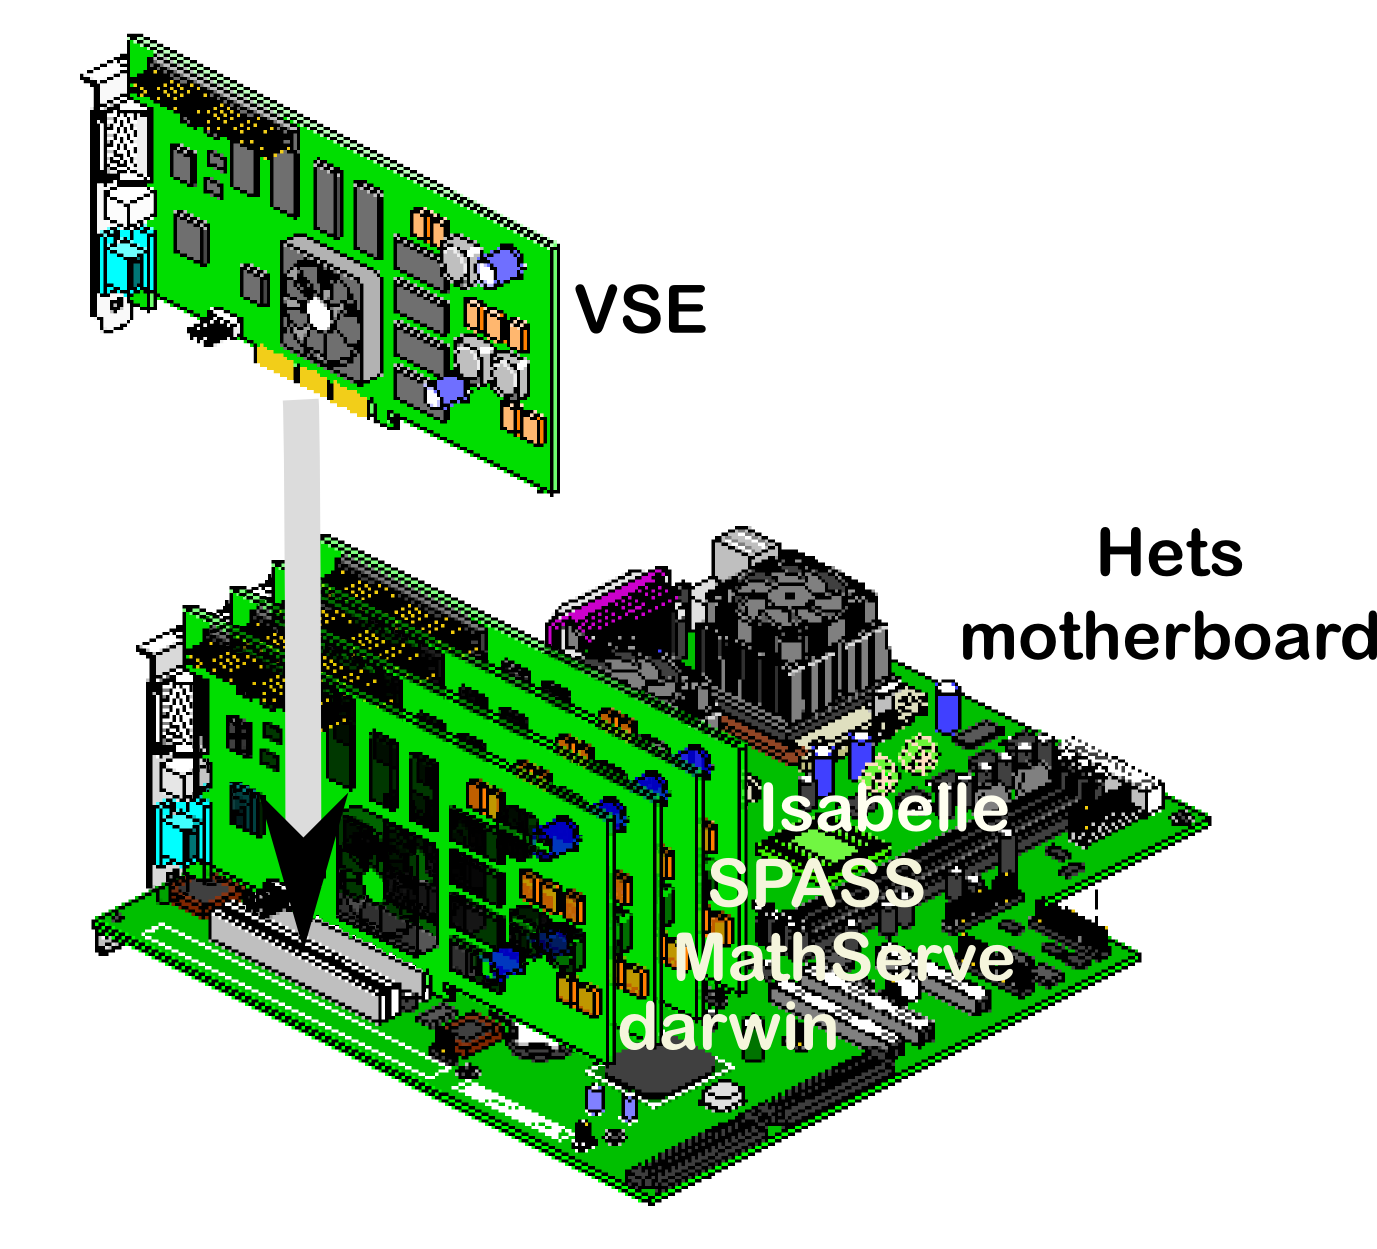
\includegraphics[width=0.45\textwidth]{hets-motherboard}
\end{center}
\caption{The \Hets motherboard and some expansion cards}
\end{figure}

\Hets supports a number of input languages directly, such as \CASL,
Common Logic, OWL-DL, Haskell, and Maude. For heterogeneous
specification, \Hets offers language heterogeneous \CASL.
Heterogeneous \CASL (\HetCASL) generalises the structuring
constructs of
\CASL \cite{CASL-UM,CASL/RefManual} to arbitrary logics
(if they are formalised as institutions and plugged into
the \Hets motherboard), as well as to heterogeneous
combination of specification written in different logics.
See
Fig.~\ref{fig:lang} for a simple subset of the
\HetCASL syntax, where \emph{basic specifications} are unstructured
specifications or modules written in a specific logic.  The graph of
currently supported logics and logic translations (the latter are also
called comorphisms) is shown in Fig.~\ref{fig:LogicGraph}, and the
degree of support by \Hets in Fig.~\ref{fig:Languages}.

\begin{figure}[ht]
\centering
{\small
\begin{verbatim}
SPEC ::= BASIC-SPEC
       | SPEC then SPEC
       | SPEC then %implies SPEC
       | SPEC with SYMBOL-MAP
       | SPEC with logic ID

DEFINITION ::= logic ID
             | spec ID = SPEC end
             | view ID : SPEC to SPEC = SYMBOL-MAP end
             | view ID : SPEC to SPEC = with logic ID end

LIBRARY = DEFINITION*
\end{verbatim}
}
\caption{Syntax of a simple subset of the heterogeneous
specification language.
\texttt{BASIC-SPEC} and \texttt{SYMBOL-MAP} have a logic
specific syntax, while \texttt{ID} stands for some form of
identifiers.\label{fig:lang}
}
\end{figure}

With \emph{heterogeneous structured specifications}, it is possible to
combine and rename specifications, hide parts thereof, and also
translate them to other logics. \emph{Architectural specifications}
prescribe the structure of implementations.  \emph{Specification
  libraries} are collections of named structured and architectural
specifications.

\Hets consists of logic-specific tools for the parsing and static
analysis of the different involved logics, as well as a
logic-independent parsing and static analysis tool for structured and
architectural specifications and libraries. The latter of course needs
to call the logic-specific tools whenever a basic specification is
encountered.

\Hets is based on the theory of institutions \cite{GoguenBurstall92},
which formalize the notion of a logic. The theory behind \Hets is laid
out in \cite{Habil}. A short overview of \Hets is given in
\cite{MossakowskiEA06,MossakowskiEtAl07b}.


\section{Logics supported by Hets}

The following list of logics (formalized as so-called institutions
\cite{GoguenBurstall92}) is currently supported by \Hets:

\begin{figure}
  \begin{center}
    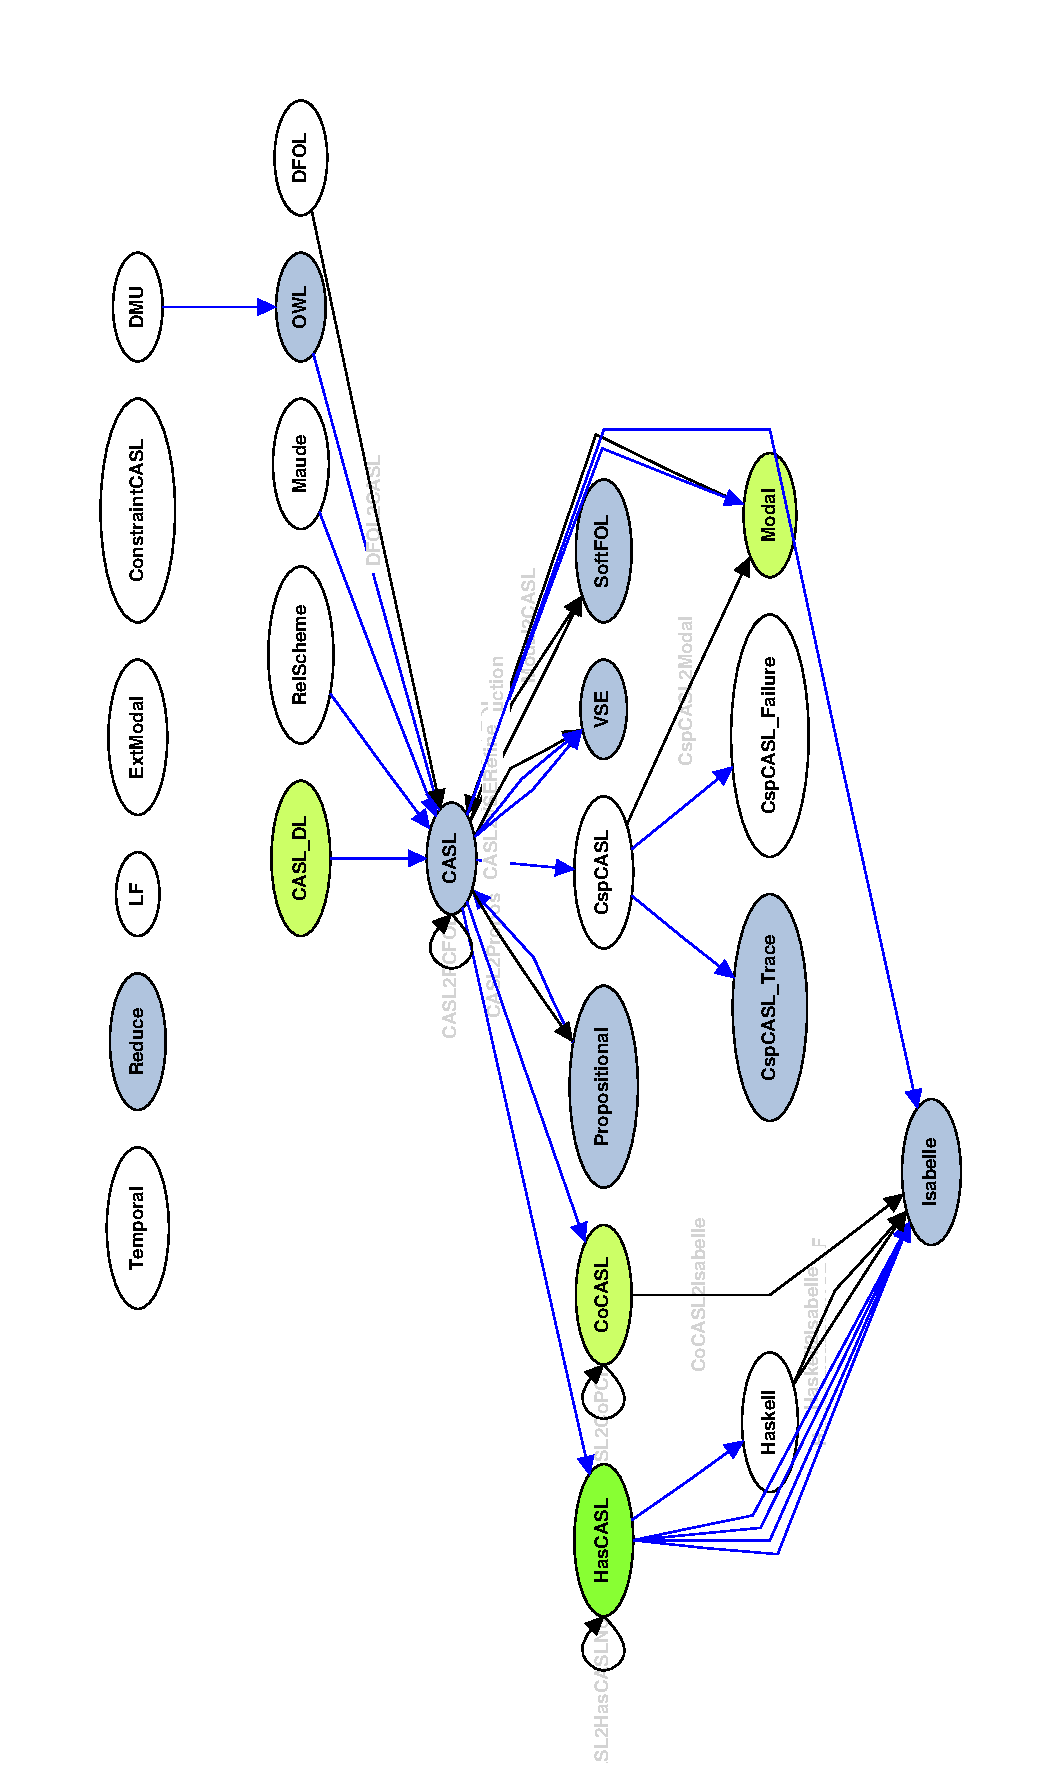
\includegraphics[scale=0.4]{LogicGraph}
  \end{center}
\caption{Graph of logics currently supported by \Hets. The more an
ellipse is filled with green, the more stable is the implementation of the logic. Blue indicates a prover-supported logic.}
\label{fig:LogicGraph}
\end{figure}


\begin{figure}
\begin{center}
\begin{tabular}{|l|c|c|c|}\hline
Language & Parser & Static Analysis & Prover \\\hline
\CASL & x & x & - \\\hline
\CoCASL & x & x & - \\\hline
\ModalCASL & x & x & - \\\hline
\HasCASL & x & x & - \\\hline
Haskell & (x) & x & - \\\hline
\CspCASL & x & x & - \\\hline
\CspCASL\_Trace & - & - & x \\\hline
\CspCASL\_Failure & - & - & - \\\hline
Constraint\CASL & x & (x) & - \\\hline
Temporal & x & (x) & - \\\hline
RelScheme & x & (x) & - \\\hline
DFOL & x & (x) & - \\\hline
ExtModal & x & (x) & - \\\hline
LF & x & (x) & - \\\hline
%Structured specifications & x & x & (x) \\\hline
%Architectural specifications & x & x & -\\\hline
\CASLDL & x & - & - \\\hline
DMU & x & - & - \\\hline
OWL DL & x & x & - \\\hline
Propositional & x & x & x \\\hline
SoftFOL & x & - & x \\\hline
Maude & x & x & - \\\hline
VSE & x & x & x \\\hline
\Isabelle & (x) & - & x \\\hline
\end{tabular}
\end{center}
\caption{Current degree of \Hets support for the different languages.\label{fig:Languages}}
\end{figure}

\begin{description}

\item[CASL] extends many sorted first-order logic with partial
  functions and subsorting.  It also provides induction sentences,
  expressing the (free) generation of datatypes.
%It is mainly designed and used for the
%specification of requirements for software systems. But it is also
%used for the specification of \Dolce (Descriptive Ontology for
%Linguistic and Cognitive Engineering), an Upper Ontology for knowledge
%representation. \cite{Gangemi:2002:SOD} Further it is now used to
%specify calculi for time and space.
For more details on \CASL see \cite{CASL/RefManual,CASL-UM}.
%
We have implemented the \CASL logic in such a way that much of the
implementation can be re-used for \CASL extensions as well; this
is achieved via ``holes'' (realized via polymorphic variables) in the
types for signatures, morphisms, abstract syntax etc.  This eases
integration of \CASL extensions and keeps the effort of integrating
\CASL extensions quite moderate.

\item[CoCASL] \cite{MossakowskiEA04} is a coalgebraic extension of \CASL,
suited for the specification of process types and reactive systems.
The central proof method is coinduction.

\item[ModalCASL] \cite{ModalCASL}
 is an extension of \CASL with multi-modalities and
term modalities. It allows the specification of modal systems with
Kripke's possible worlds semantics. It is also possible to express
certain forms of dynamic logic.

\item[HasCASL] is a higher order extension of \CASL allowing
  polymorphic datatypes and functions. It is closely related to the
  programming language Haskell and allows program constructs being
  embedded in the specification.
  An overview of \HasCASL is given in \cite{Schroeder:2002:HIS};
the language is summarized in \cite{HasCASL/Summary}, the semantics
in \cite{Schroder05b,Schroder-habil}.

\item[Haskell] is a modern, pure and strongly typed functional
  programming language. It simultaneously is the implementation
  language of \Hets, such that in the future, \Hets might be applied
  to itself.
The definitive reference for Haskell is \cite{PeytonJones03},
see also \url{www.haskell.org}.

\item[CspCASL] \cite{Roggenbach06} is a combination of \CASL
  with the process algebra CSP.

\item[ConstraintCASL] is an experimental logic for the specification
of qualitative constraint calculi.

\item[OWL DL] is the Web Ontology Language (OWL) recommended by the
  World Wide Web Consortium (W3C, \url{http://www.w3c.org}). It is
  used for knowledge representation and the Semantic Web
  \cite{berners:2001:SWeb}.
Hets calls an external OWL DL parser
  written in JAVA to obtain the abstract syntax for an OWL file and its
  imports. The JAVA parser is also doing a first analysis classifying
  the OWL ontology into the sublanguages OWL Full, OWL DL and OWL
  Lite.
 Hets only supports the last two, more restricted variants.
The
  structuring of the OWL imports is displayed as Development Graph.

\item[CASL-DL] \cite{OWL-CASL-WADT2004}
is an extension of a restriction of \CASL, realizing
a strongly typed variant of OWL DL in \CASL syntax.
It extends
  \CASL with cardinality restrictions for the description of sorts and
  unary predicates. The restrictions are based on the equivalence
  between \CASLDL, OWL~DL and \SHOIN. Compared to \CASL only unary
  and binary predicates, predefined datatypes and concepts (subsorts
  of the topsort Thing) are allowed. It is used to bring OWL DL and
  \CASL closer together.

\item[Propositional] is classical propositional logic, with
the zChaff SAT solver \cite{Herbstritt03} connected to it.

\item[SoftFOL] \cite{LuettichEA06a} offers three automated theorem
  proving (ATP) systems for first-order logic with equality: (1) \SPASS
  \cite{WeidenbachEtAl02}; (2) Vampire \cite{RiazanovV02}; and (3)
  MathServe Broker\footnote{which chooses an appropriate ATP upon a
    classification of the FOL problem} \cite{ZimmerAutexier06}.
  These together comprise some of the most advanced theorem provers
  for first-order logic.

\item[\Isabelle] \cite{NipPauWen02} is an interactive theorem prover
  for higher-order logic.
\end{description}
\ednote{TODO Till: update list}

Various logics are supported with proof tools. Proof support for the
other logics can be obtained by using logic translations to a
prover-supported logic.


An introduction to \CASL can be found in the \CASL User Manual
\cite{CASL-UM}; the detailed language reference is given in
the \CASL Reference Manual \cite{CASL/RefManual}.  These documents
explain both the \CASL logic and language of basic specifications as
well as the logic-independent constructs for structured and
architectural specifications.  The corresponding document explaining the
\HetCASL language constructs for \emph{heterogeneous} structured specifications
is the \HetCASL language summary \cite{Mossakowski04}; a formal
semantics as well as a user manual with more examples are in preparation.
Some of \HetCASL's heterogeneous constructs will be illustrated
in Sect.~\ref{sec:HetSpec} below.

\section{Logic translations supported
by Hets}
\label{comorphisms}

Logic translations (formalized as institution comorphisms
\cite{GoguenRosu02}) translate from a given source logic to a given
target logic. More precisely, one and the same logic translation
may have several source and target \emph{sub}logics: for
each source sublogic, the corresponding sublogic of the target
logic is indicated.
A graph of the most important logics and sublogics, together with their
comorphisms, is shown in Fig.~\ref{fig:SublogicGraph}.

\begin{figure}
  \begin{center}
    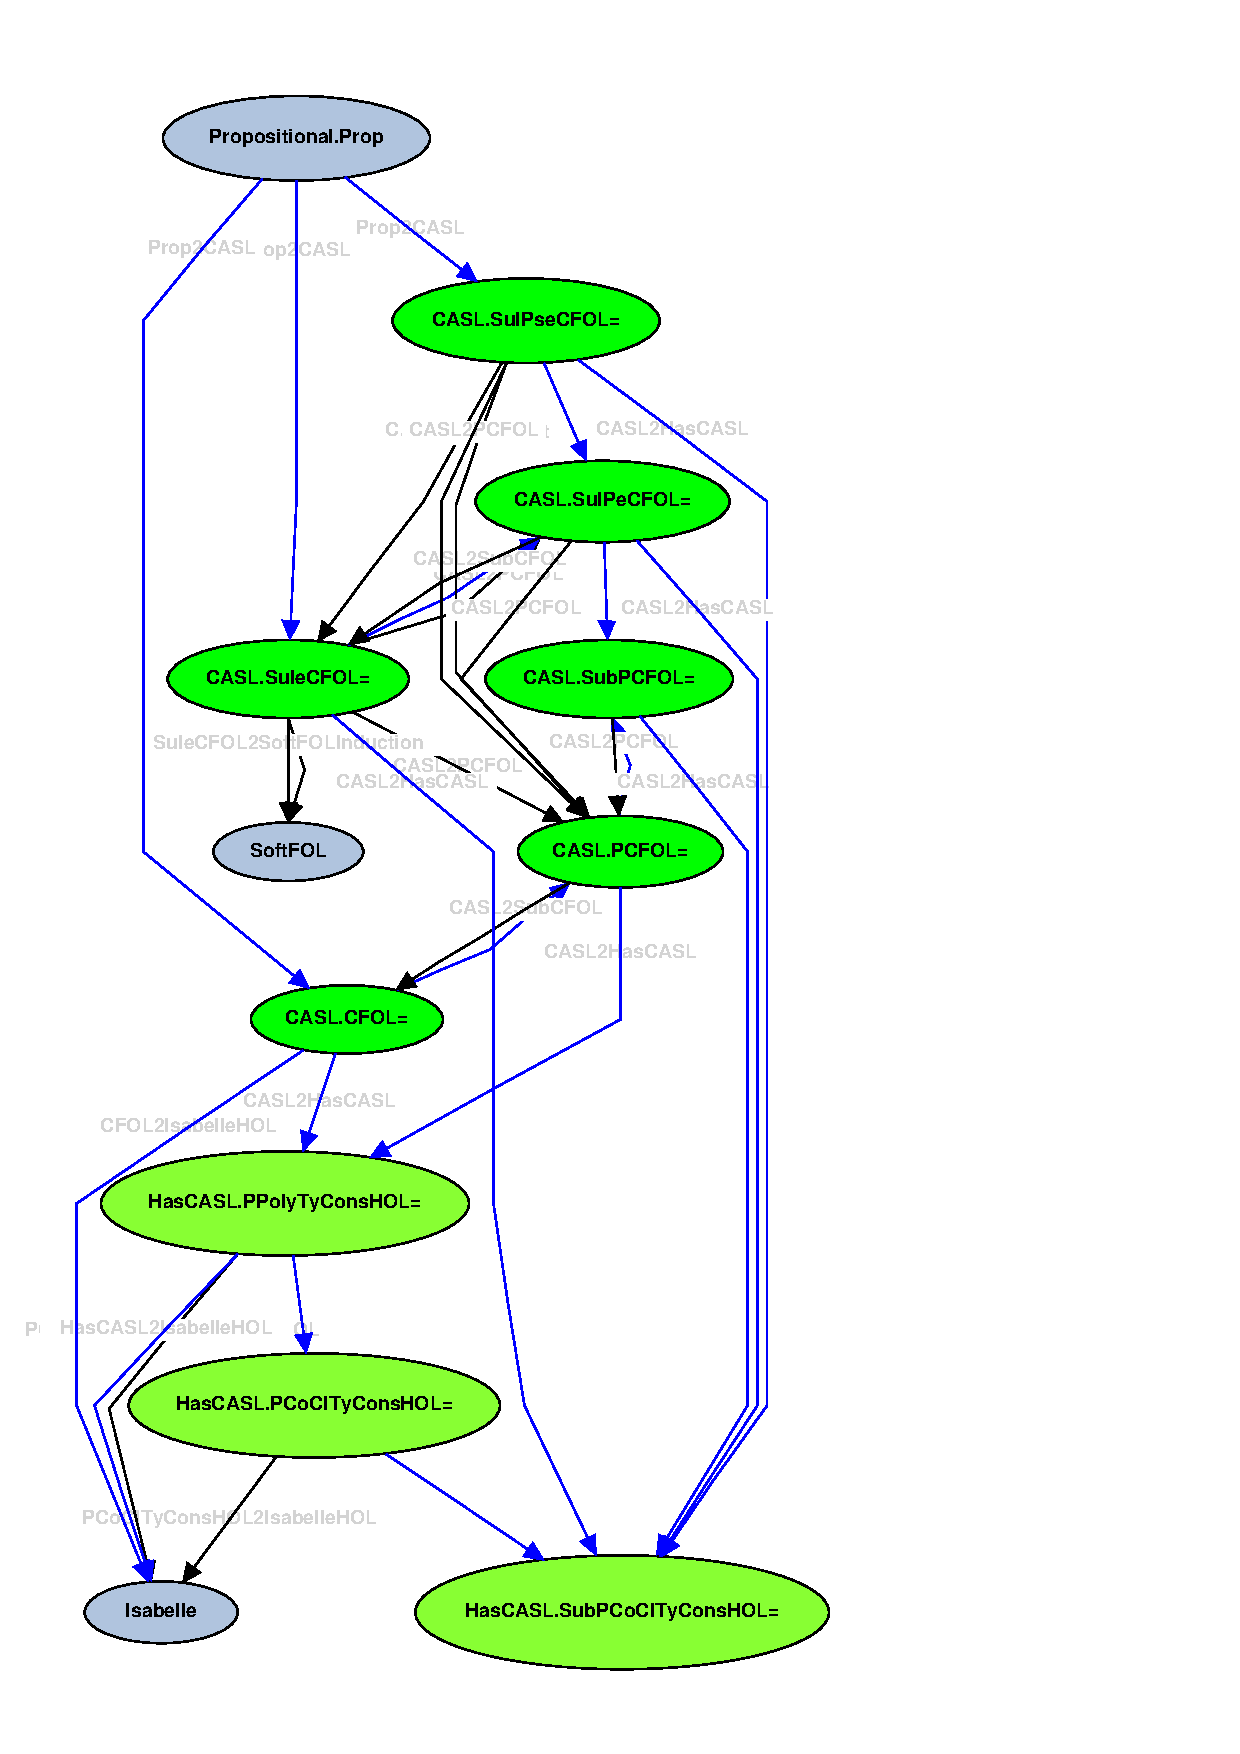
\includegraphics[scale=0.4]{SublogicGraph}
  \end{center}
\caption{Graph of most important sublogics currently supported by \Hets,
together with their comorphisms.}
\label{fig:SublogicGraph}
\end{figure}

In more detail, the following list of logic translations is currently
supported by \Hets:
\ednote{TODO Mihai,Till: check VSE, Maude, DFOL descr. or ref.}

\begin{tabular}{|l|p{8cm}|}\hline
CASL2CoCASL & inclusion \\\hline
CASL2CspCASL & inclusion \\\hline
CASL2HasCASL & inclusion \\\hline
CASL2Isabelle & inclusion on sublogic CFOL=
(translation $(7)$ of \cite{Mossakowski02}) \\\hline
CASL2Modal & inclusion \\\hline
CASL2PCFOL & coding of subsorting (SubPCFOL=) by injections, see Chap.\ III:3.1 of the CASL Reference Manual \cite{CASL/RefManual} \\\hline
CASL2PCFOLTopSort & coding of subsorting (SulPeCFOL=) by a top sort and unary
predicates for the subsorts \\\hline
CASL2Propositional & translation of propositional FOL \\\hline
CASL2SoftFOL & coding of CASL.SuleCFOL=E to SoftFOL \cite{LuettichEA06a},
mapping types to soft types \\\hline
CASL2SoftFOLInduction & same as CASL2SoftFOL but with instances of induction
axioms for all proof goals \\\hline
CASL2SubCFOL & coding of partial functions by error elements
(translation $(4a')$ of \cite{Mossakowski02}, but extended to subsorting, i.e. sublogic SubPCFOL=) \\\hline
CASL2VSE & inclusion on sublogic CFOL= \\\hline
CASL2VSEImport & inclusion on sublogic CFOL= \\\hline
CASL2VSERefine & refining translation of CASL.CFOL= to VSE \\\hline
CASL\_DL2CASL & inclusion \\\hline
CoCASL2CoPCFOL & coding of subsorting by injections, similar to CASL2PCFOL \\\hline
CoCASL2CoSubCFOL & coding of partial functions by error supersorts, similar to  CASL2SubCFOL \\\hline
CoCASL2Isabelle & extended translation similar to CASL2Isabelle \\\hline
CspCASL2CspCASL\_Failure & inclusion \\\hline
CspCASL2CspCASL\_Trace & inclusion \\\hline
CspCASL2Modal & translating the CASL data part to ModalCASL \\\hline
DFOL2CASL & translating dependent types \\\hline
DMU2OWL & interpreting Catia output as OWL \\\hline
\end{tabular}

\begin{tabular}{|l|p{7cm}|}\hline
HasCASL2HasCASLNoSubtypes & coding out subtypes \\\hline
HasCASL2HasCASLPrograms & coding of \HasCASL axiomatic recursive definitions
as \HasCASL recursive program definitions \\\hline
HasCASL2Haskell & translation of \HasCASL recursive program definitions to Haskell \\\hline
HasCASL2IsabelleOption & coding of HasCASL to Isabelle/HOL \cite{Groening05} \\\hline
Haskell2Isabelle & coding of Haskell to Isabelle/HOL \cite{TorriniEtAl07} \\\hline
Haskell2IsabelleHOLCF & coding of Haskell to Isabelle/HOLCF \cite{TorriniEtAl07} \\\hline
Maude2CASL & inclusion \\\hline
Modal2CASL & the standard translation of modal logic
to first-order logic \cite{blackburn_p-etal:2001a} \\\hline
OWL2CASL & inclusion \\\hline
Propositional2CASL & inclusion \\\hline
RelScheme2CASL & inclusion \\\hline
\end{tabular}

\section{Getting started}

The latest \Hets version can be obtained from the
\Hets tools home page
\begin{quote}
\url{http://www.dfki.de/sks/hets}
\end{quote}
 Since \Hets is being
improved constantly, it is recommended always to use the latest version.

\Hets currently is available (on Intel architectures only) for Linux, Solaris
and Mac OS-X.

There are three possibilities to install \Hets:
\begin{enumerate}
\item
The Java-based \Hets installer. Download a \texttt{.jar} file and
start it with
\begin{quote}
java -jar \texttt{file.jar}
\end{quote}
Note that you need Sun Java 1.4.2 or later. On a Mac, you can just
double-click on the \texttt{.jar} file.

The installer will lead you through the installation with
a graphical interface. It will download and install further
software (if not already installed on your computer):

\medskip
{\small
\begin{tabular}{|l|l|p{5cm}|}\hline
Hets-lib & specification library & \url{http://www.cofi.info/Libraries}\\\hline
uDraw(Graph) & graph drawing & \url{http://www.informatik.uni-bremen.de/uDrawGraph/en/}\\\hline
Tcl/Tk & graphics widget system & (version 8.4 or 8.5 must be installed before)\\\hline
\SPASS & theorem prover & \url{http://spass.mpi-sb.mpg.de/}\\\hline
Darwin & theorem prover & should be installed manually from \url{http://combination.cs.uiowa.edu/Darwin/}\\\hline
\Isabelle & theorem prover & \url{http://www.cl.cam.ac.uk/Research/HVG/Isabelle/}\\\hline
(X)Emacs & editor (for Isabelle) & (must be installed manually)\\\hline
\end{tabular}
}
\medskip

\item
If you do not have Sun Java, you can just download the hets binary.
You have to unpack it with \texttt{bunzip2} and then put it at
some place coverd by your \texttt{PATH}. You also have to
install the above mentioned software and set
several environment variables, as explained on the installation page.

\item
You may compile \Hets from the sources, please follow the
link ``Hets: source code and information for developers''
on the \Hets web page, download the sources (as tarball or from
svn), and follow the
instructions in the \texttt{INSTALL} file, but be prepared to take some time.
\end{enumerate}

Depending on your application further tools are supported and may be
installed in addition:

\medskip
{\small
\begin{tabular}{|l|l|p{5cm}|}\hline
zChaff & SAT solver & \url{http://www.princeton.edu/~chaff/zchaff.html} \\\hline
minisat & SAT solver & \url{http://minisat.se/} \\\hline
Pellet & OWL reasoner & \url{http://clarkparsia.com/pellet/} \\\hline
E-KRHyper & theorem prover
  & \url{http://userpages.uni-koblenz.de/~bpelzer/ekrhyper/} \\\hline
Reduce & computer algebra system
  & \url{http://www.reduce-algebra.com/} \\\hline
Maude & rewrite system & \url{http://maude.cs.uiuc.edu/} \\\hline
VSE & theorem prover & (non-public) \\\hline
Twelf & & \url{http://twelf.plparty.org/} \\\hline
\end{tabular}
}
\ednote{TODO Mihai, Till, Luecke: check prover list}


\section{Analysis of Specifications}
Consider the following \CASL
specification:

\medskip
\begin{BIGEXAMPLE}
\I\SPEC \NAME{Strict\_Partial\_Order} =
%%PDM\I{}    \COMMENTENDLINE{Let's start with a simple example !}
\begin{ITEMS}[\PRED]
\I\SORT    \( Elem \)
\I\PRED    \( \_\_<\_\_ : Elem \* Elem \)
%           \COMMENTENDLINE{\PRED abbreviates predicate}
\end{ITEMS}
\(\[  \FORALL x,y,z : Elem \\
      \. \NOT(x < x)                      \RIGHT{\LABEL{strict}}     \\
      \. x < y   \IMPLIES  \NOT(y < x)    \RIGHT{\LABEL{asymmetric}} \\
      \. x < y \A y < z  \IMPLIES  x < z  \RIGHT{\LABEL{transitive}} \\
\]\)
\begin{COMMENT}
Note that there may exist \(x, y\) such that\\
neither \(x < y\) nor \(y < x\).
\end{COMMENT}
\I\END
\end{BIGEXAMPLE}

\Hets can be used for parsing and
checking static well-formedness of specifications.

                \index{parsing}%
                \index{static!analysis}%
                \index{analysis, static}%

Let us assume that the example is in a file named
\texttt{Order.casl} (actually, this file is provided
with the \Hets distribution as \texttt{Hets-lib/UserManual/Chapter3.casl}).
Then you can check the well-formedness of the
specification by typing (into some shell):

\begin{quote}
\texttt{hets Order.casl}
\end{quote}
\Hets checks both the correctness of this specification
 with respect to the \CASL syntax, as
well as its correctness with respect to the static semantics (e.g.\
whether all identifiers have been declared before they are used,
whether operators are applied to arguments of the correct sorts,
whether the use of overloaded symbols is unambiguous, and so on).
The following flags are available in this context:
\begin{description}
\item[\texttt{-p}, \texttt{--just-parse}] Just do the parsing
 -- the static analysis is skipped and no development is created.
\item[\texttt{-s}, \texttt{--just-structured}] Do the parsing and the
  static analysis of (heterogeneous) structured specifications, but
  leave out the analysis of basic specifications.  This can be used
  for prototyping issues, namely to quickly produce a development graph
  showing the dependencies among the specifications (cf.
  Sect.~\ref{sec:DevGraph}) even if the individual specifications are
  not correct yet.
\item[\texttt{-L DIR}, \texttt{--hets-libdir=DIR}]
Use \texttt{DIR} as a colon separated list of directories for specification libraries (equivalently, you can set the variable \texttt{HETS\_LIB} before
calling \Hets).
\item[\texttt{-a ANALYSIS}, \texttt{--casl-amalg=ANALYSIS}]
  For the analysis of architectural specification (a quite advanced
  feature of \CASL), the \texttt{ANALYSIS} argument specifies the options for
  amalgamability checking
  algorithm for \CASL logic; it is a comma-separated list of zero or
  more of the following options:
  \begin{description}
  \item[\texttt{sharing}] perform sharing analysis for sorts,
    operations and predicates.
  \item[\texttt{cell}] perform cell condition check; implies
    \texttt{sharing}. With this option on, the subsort embeddings are
    analyzed.
  \item[\texttt{colimit-thinness}] perform colimit thinness check;
    implies \texttt{sharing}. The colimit thinness check is less
    complete and usually takes longer than the full cell condition
    check (\texttt{cell} option), but may prove more efficient in case
    of certain specifications.
  \end{description}
  If \texttt{ANALYSIS} is empty then amalgamability analysis for
  \CASL is skipped.
  The default value for \texttt{--casl-amalg} is
  \texttt{cell}.
\end{description}

\section{Heterogeneous Specification} \label{sec:HetSpec}

\Hets accepts plain text input files with the following endings:
\\

\begin{tabular}{|l|c|c|}\hline
Ending & default logic & structuring language\\\hline
\texttt{.casl} & \CASL & \CASL \\\hline
\texttt{.het} & \CASL & \CASL \\\hline
\texttt{.hs} & Haskell & Haskell\\\hline
\texttt{.owl} & OWL DL, OWL Lite & OWL\\\hline
\texttt{.elf} & LF & Twelf \\\hline
\texttt{.maude} & Maude & Maude \\\hline
\end{tabular}

\medskip

Furthermore, \texttt{.xml} files are accepted as Catia output if the default
logic is set to DMU before a library import or by the ``\texttt{-l DMU}''
command line option of \Hets.

Although the endings \texttt{.casl} and \texttt{.het} are
interchangeable, the former should be used for libraries of
homogeneous \CASL specifications and the latter for \HetCASL libraries
of heterogeneous specifications (that use the \CASL structuring
constructs). Within a \HetCASL library, the current logic can be changed e.g.\
to \HasCASL in the following way:

\begin{verbatim}
logic HasCASL
\end{verbatim}

The subsequent specifications are then parsed and analysed as
\HasCASL specifications. Within such specifications,
it is possible to use references to named \CASL specifications;
these are then automatically translated along the default
embedding of \CASL into \HasCASL (cf.\ Fig.~\ref{fig:LogicGraph}).
(There are also heterogeneous constructs
for explicit translations between logics, see \cite{Mossakowski04}.)

\eat{
A \CspCASL specification consists of a \CASL specification
for the data part and a \Csp process built over this data part.
Therefore, \HetCASL provides a heterogeneous language construct
\texttt{data} as follows:

\begin{verbatim}
library Buffer

logic CASL

spec List =
  free type List[Elem] ::= nil | cons(Elem; List[Elem])
  ops last: List -> ? Elem;
      rest: List -> ? List
end

logic CspCASL

spec Buffer =
  data List
  channel read, write : Elem
  process Buf(List): read, write, List;
          EmptyBuffer : read,write, List;
          Buf(l)= read? x :: Elem -> Buf(cons(x,nil)) []
                  (if l=nil then STOP else
                   write!last(l) -> Buf(rest(l)))
          EmptyBuffer = Buf(nil)
end
\end{verbatim}

Here, the construct \texttt{data List} refers to the \CASL specification
\texttt{List}, which is implicitly embedded into \CspCASL.
}

The ending \texttt{.hs} is available for directly reading in
Haskell programs % and HasSLe specifications,
and hence supports the Haskell module system.
By contrast, in \HetCASL libraries (ending with \texttt{.het}),
the logic Haskell has to be chosen explicitly, and the \CASL structuring
syntax needs to be used:

\begin{verbatim}
library Factorial

logic Haskell

spec Factorial =
{
fac :: Int -> Int
fac n = foldl (*) 1 [1..n]
}
end
\end{verbatim}

Note that according to the Haskell syntax, Haskell function
declarations and definitions need to start with the first column of
the text.




\section{Development Graphs}\label{sec:DevGraph}

Development graphs are a simple kernel formalism for (heterogeneous)
structured theorem proving and proof management.

A development graph consists of a set of nodes (corresponding to whole
structured specifications or parts thereof), and a set of arrows
called \emph{definition links}, indicating the dependency of each
involved structured specification on its subparts.  Each node is
associated with a signature and some set of local axioms.  The axioms
of other nodes are inherited via definition links.  Definition links
are usually drawn as black solid arrows, denoting an import of another
specification.

Complementary to definition links, which \emph{define} the theories of
related nodes, \emph{theorem links} serve for \emph{postulating}
relations between different theories. Theorem links are the central
data structure to represent proof obligations arising in formal
developments.
Theorem links can be \emph{global} (drawn as solid arrows) or
\emph{local} (drawn as dashed arrows): a global theorem link
postulates that all axioms of the source node (including the inherited
ones) hold in the target node, while a local theorem link only postulates
that the local axioms of the source node hold in the target node.

Both definition and theorem links can be \emph{homogeneous},
i.e. stay within the same logic, or \emph{heterogeneous}, i.e.\ %% such that
the logic changes along the arrow. Technically, this is the case
for Grothendieck signature morphisms $(\rho,\sigma)$ where
$\rho\not=id$. This case is indicated with double arrows.

Theorem links are initially displayed in red.
The \emph{proof
  calculus} for development graphs
\cite{MossakowskiEtAl05,Habil} is given by rules
that allow for proving global theorem links by decomposing them
into simpler (local and global) ones. Theorem links that have been
proved with this calculus are drawn in green. Local theorem links can
be proved by turning them into \emph{local proof goals}.  The latter
can be discharged using a logic-specific calculus as given by an
entailment system for a specific institution. Open local
proof goals are indicated by marking the corresponding node in the
development graph as red; if all local implications are proved, the
node is turned into green. This implementation ultimately is based
on a theorem \cite{Habil} stating soundness and relative completeness
of the proof calculus for heterogeneous development graphs.

Details can be found in the \CASL Reference Manual \cite[IV:4]{CASL/RefManual}
and in \cite{Habil,MossakowskiEtAl05,MossakowskiEtAl07b}.

The following options let \Hets show the development graph of
a specification library:
\begin{description}
\item[\texttt{-g}, \texttt{--gui}] Shows the development graph in a GUI window
\item[\texttt{-u}, \texttt{--uncolored}] no colors in shown graphs
\end{description}

The following additional options also apply typical rules from the development
graph calculus to the final graph and save applying these rule via the GUI.
\begin{description}
\item[\texttt{-A}, \texttt{--apply-automatic-rule}] apply the automatic
  strategy to the development graph. This is what you usual want in order to
  get goals within nodes for proving.
\item[\texttt{-N}, \texttt{--normal-form}] compute all normal forms for nodes
  with incoming hiding links. (This may take long and may not be implemented
  for all logics.)
\end{description}

\eat{
Let us extend the above library \texttt{Order.casl}. One use of the
library might be to express the fact that the natural numbers form a
strict partial order as a view, as follows:

\medskip
\begin{BIGEXAMPLE}
\I\SPEC \NAMEREF{Natural} = ~\FREE \TYPE \(Nat ::= 0 \| suc(Nat)\)~\END
\end{BIGEXAMPLE}


\begin{EXAMPLE}
\I\SPEC \NAMEDEFN{Natural\_Order\_2} =
\IEXT{\NAMEREF{Natural}} \THEN
\begin{ITEMS}
\I\PRED \( \_\_<\_\_ : Nat \* Nat\)
\end{ITEMS}
\(\[    \FORALL x,y:Nat \\
        \. 0 < suc(x) \\
        \. \neg x < 0 \\
        \. suc(x) < suc(y) \IFF x < y
\]\)
\I\END
\end{EXAMPLE}

\begin{EXAMPLE}%[\SLIDESMALL]
\I\VIEW \NAMEDEFN{v1} ~:~ \NAMEREF{Strict\_Partial\_Order}  \TO
\NAMEREF{Natural\_Order\_2} =
\I{} \( Elem \MAPSTO Nat\)
\I\END
\end{EXAMPLE}

Again, these specifications can be checked with \Hets. However, this
only checks syntactic and static semantic well-formedness -- it is
\emph{not} checked whether the predicate `$\_\_<\_\_$' introduced in
\NAMEREF{Natural\_Order\_2} actually is constrained to be interpreted
by a strict partial ordering relation. Checking this requires theorem
proving, which will be discussed below.

However, before coming to theorem proving, let us first inspect the
proof obligations arising from a specification.  This can be done with:
\begin{quote}
\texttt{hets -g Order.casl}
\end{quote}
(assuming that the above two specifications and the view
have been added to the file
\texttt{Order.casl}).
\Hets now displays a so-called development graph
(which is just an overview graph showing the overall structure
of the specifications in the library), see Fig.~\ref{fig:dg0}.


\begin{figure}
\begin{center}
\includegraphics[scale=0.7]{dg-order-0}
\end{center}
\caption{Sample development graph.\label{fig:dg0}}
\end{figure}

Nodes in a development graph correspond to \CASL specifications.
Arrows show how specifications are related by the structuring
constructs.

The black arrow denotes an ordinary import of
specifications (generated by the extension), while the red arrow
denotes a proof obligation (corresponding to the view).
This proof obligation needs to be discharged in order to
show that the view is well-formed (then its color turns into green).

As a more complex example, consider the following loose specification
of a sorting function, taken from the \CASL User Manual
\cite{CASL-UM}, Chap.~6:

\begin{BIGEXAMPLE}
\I\SPEC \NAMEREF{List\_Order\_Sorted}
\\{} [\,\NAMEREF{Total\_Order} \WITH \SORT \(Elem\), \PRED \(\_\_<\_\_\)\,] =
\IEXT{\NAMEREF{List\_Selectors} [\,\SORT \(Elem\)\,]} \THEN
\begin{ITEMS}[\WITHIN]
\I\LOCAL
\begin{ITEMS}[\PRED]
\I\PRED  \( \_\_is\_sorted : List \)
\end{ITEMS}
\(\[  \FORALL e,e': Elem; L : List \\
      \. empty~is\_sorted \\
      \. cons(e,empty)~is\_sorted \\
      \. cons(e,cons(e',L))~is\_sorted \IFF
\\\M         (cons(e',L)~is\_sorted \A \NOT(e'<e)) \]\)
\I\WITHIN
\begin{ITEMS}[\OP]
\I\OP    \( order : List \TOTAL List \)
\end{ITEMS}
\( \FORALL L:List\. \[ order(L)~is\_sorted \]\)
\end{ITEMS}
\I\END
\end{BIGEXAMPLE}

The following specification of sorting by insertion also is taken from
the \CASL User Manual \cite{CASL-UM}, Chap.~6:

\begin{BIGEXAMPLE}
\I\SPEC \NAMEREF{List\_Order}
      [\,\NAMEREF{Total\_Order} \WITH \SORT \(Elem\), \PRED \(\_\_<\_\_\)\,] =
\phantomsection
\IEXT{\NAMEREF{List\_Selectors} [\,\SORT \(Elem\)\,]} \THEN
\begin{ITEMS}[\WITHIN]
\I\LOCAL
\begin{ITEMS}[\OP]
\I\OP    \( insert : Elem \* List \TOTAL List \)
\end{ITEMS}
\(\[  \FORALL e,e':Elem; L:List \\
      \. insert(e, empty) = cons(e, empty) \\
      \. insert(e, cons(e',L)) = \[ cons(e', insert(e,L)) \WHEN e' < e\\
                                    \ELSE cons(e, cons(e',L)) \] \\
\]\)
\I\WITHIN
\begin{ITEMS}[\OP]
\I\OP    \( order : List \TOTAL List \)
\end{ITEMS}
\(\[  \FORALL e:Elem; L:List \\
      \. order(empty) = empty \\
      \. order(cons(e,L)) = insert(e, order(L))  \]\)
\end{ITEMS}
\I\END
\end{BIGEXAMPLE}


Both specifications are related. To see this, we first inspect
their signatures. This is possible with:
\begin{quote}
\texttt{hets -g Sorting.casl}
\end{quote}
assuming that \texttt{Sorting.casl} contains the above specifications.
\Hets now displays a more complex development graph, see Fig.~\ref{fig:dg1}.


\begin{figure}
\begin{center}
\includegraphics[scale=0.7]{dg-order-1}
\end{center}
\caption{Development graph for the two sorting specifications.\label{fig:dg1}}
\end{figure}


In the above-mentioned development graph, we have two types of nodes.
The named ones correspond to named specifications, but there
are also unnamed nodes corresponding to anonymous basic
specifications like the declaration of the $insert$ operation in
\NAMEREF{List\_Order} above. Basically, there is an
unnamed node for each structured specification that is not named.

Again, the black arrows denote an ordinary import of specifications
(corresponding to the extensions and unions in the
specifications), while the blue arrows denote hiding (corresponding to
the local specification).

By clicking on the nodes, one can inspect their signatures.
In this way, we can see that both  \NAMEREF{List\_Order\_Sorted}  and
\NAMEREF{List\_Order} have the same signature. Hence, it
is legal to add a view:

\begin{EXAMPLE}%[\SLIDESMALL]
\I\VIEW \NAMEDEFN{v2}[\NAMEREF{Total\_Order}] ~:~ \NAMEREF{List\_Order\_Sorted}[\NAMEREF{Total\_Order}]  \TO
\NAMEREF{List\_Order}[\NAMEREF{Total\_Order}]
\I\END
\end{EXAMPLE}

We have already added this view to \texttt{Sorting.casl}.
The corresponding
proof obligation between \NAMEREF{List\_Order\_Sorted}  and
\NAMEREF{List\_Order} is displayed in Fig.~\ref{fig:dg1}
 as a red arrow.
}

Here is a summary of the types of nodes and links occurring in
development graphs:
\begin{description}
\item[Named nodes] correspond to a named specification.
\item[Unnamed nodes] correspond to an anonymous specification.
\item[Elliptic nodes] correspond to a specification in the current library.
\item[Rectangular nodes] are external nodes corresponding to a specification
  downloaded from another library.
\item[Red nodes] have open proof obligations.
\item[Yellow nodes] have an open conservativity proof obligations.
\item[Green nodes] have all proof obligations resolved.
\item[Black links] correspond to reference to other specifications (definition
  links in the sense of \cite[IV:4]{CASL/RefManual}).
\item[Red links] correspond to open proof obligations (theorem links).
\item[Green links] correspond to proven theorem links.
\item[Yellow links] correspond to proven theorem links with open
  conservativity or to open hiding theorem links.
\item[Blue links] correspond to hiding, free, or cofree definition links.
\item[Violett links] correspond to a mixture of links becoming visible after
 ``expand'' or ``Show unnamed nodes with open proofs''.
\item[Solid links] correspond to global (definition or theorem)
links in the sense of \cite[IV:4]{CASL/RefManual}.
\item[Dashed links] correspond to local (theorem) links in the sense of
  \cite[IV:4]{CASL/RefManual}. These are usually created after
  ``Global-Decomposition'' or only be visible after ``Show newly added proven
  edges''.
\item[Single line links] have homogeneous signature morphisms (staying within
  one and the same logic).
\item[Double line links] have heterogeneous signature morphisms (moving
  between logics).
\end{description}

We now explain the menus of the development graph window.
Most of the pull-down menus of the window are uDraw(Graph)-specific
layout menus;
their function can be looked up in the uDraw(Graph) documentation\footnote{see
\url{http://www.informatik.uni-bremen.de/uDrawGraph/en/service/uDG31\_doc/}.}.
The exception is the Edit menu. Moreover, the nodes and links
of the graph have attached pop-up menus, which appear when
clicking with the right mouse button.
\ednote{TODO Mihai: update}\\

\begin{description}
\item[Edit] This menu has the following submenus:
\begin{description}
\item[undo] Undo the last development graph proof step (see under Proofs)
\item[redo] Restore the last undone development graph proof step (see
  under Proofs)
\item[Unnamed nodes]
The ``Hide/show names'' menu is a toggle:
you can switch on or off the display of names for nodes that
are initially unnamed. The newly named nodes get names that
are derived from named neighbour nodes.

With the ``Hide nodes'' submenu, it is possible
to reduce the complexity of the graph by hiding all unnamed nodes;
only nodes corresponding to named specifications remain displayed.
Paths between named nodes going through unnamed nodes
are displayed as links. With the ``Show nodes'' submenu, the unnamed
nodes re-appear.
\item[Proofs] This menu allows to apply some of the deduction rules
  for development graphs, see Sect. IV:4.4 of the \CASL Reference
  Manual \cite{CASL/RefManual} or one of
  \cite{Habil,MossakowskiEtAl05,MossakowskiEtAl07b}. While support for
  local and global (definition or theorem) links is stable, support
  for hiding links and checking conservativity is still experimental.
  In most cases, it is advisable to use ``Automatic'', which
  automatically applies the rules in the correct order. As a result,
  the the open theorem links (marked in red) will be reduced to local
  proof goals, that is, they become green, and instead, some of the
  node will get red, indicating open local proof goals.
  Besides the deduction rules, the menu contains entries for computing
  a colimit approximation for the development graph and for
  computing normal forms of all nodes (needed when dealing with hiding).
\end{description}

\item[Pop-up menu for nodes]
Here, the number of submenus depends on the type of the node:
\begin{description}
\item[Show signature] Shows the signature of the node.
\item[Show local axioms] Shows the local axioms of the node.
\item[Show theory] Shows the theory of the node (including axioms
imported from other nodes). Warning: axioms imported via hiding  links
are not part of the theory; they can be made visible only by re-adding
the hidden symbols, using the proof rule \emph{Theorem-Hide-Shift}.
\item[Translate theory] Translates the theory of a node to another logic.
A menu with the possible translation paths will be displayed.
\item[Taxonomy graphs] (Only available for some logics) Shows the subsort graph of the signature of the node.
\item[Show sublogic] Shows the logic and, within that logic, the minimal sublogic
for the signature and the axioms of the node.
\item[Show origin] Shows the kind of \CASL structuring construct that
led to the node.
\item[Show proof status] Show open and proven local proof goals.
\item[Prove] Try to prove the local proof goals. See Section~\ref{sec:Proofs}
for details.
\item[Check consistency] Check the consistency of the theory of the node.
\item[Show just subtree] (Only for named nodes) Reduce the complexity
of the graph by just showing the subtree below the current node.
\item[Undo show just subtree] (Only for named nodes) Undo the reduction.
\item[Show referenced library] (Only for external nodes) Open a new window
showing the development graph for the library the external node refers to.
%\item[Show spec] Show the structured specification of the node.
% (not fully implemented yet)
\item[Show number of node] Show the internal number of the node.
\end{description}
\item[Pop-up menu for links]
Again, the number of submenus depends on the type of the link:
\begin{description}
\item[Show morphism] Shows the signature morphism of the link. It consists
of two components: a logic translation and a signature morphism in the
target logic of the logic translation.
In the (most frequent) case
of an intra-logic signature morphism, the logic translation component is
just the identity.
\item[Show origin] Shows the kind of \CASL structuring construct that
led to the link.
\item[Show proof status] (Only for theorem links) Show the proof status.
\item[Check conservativity] (Experimental) Check whether the
theory of the target node of the link
is a conservative extension of the theory of the source node.
\item[Show ID of this edge] Shows the internal number of the edge.
These numbers are also used in the proof status information for
edges.
\end{description}
\end{description}

Besides development graphs there are library graph windows displaying the
library hierarchy. The Edit menu has the following submenus:

\begin{description}
\item[Edit] This menu for library graphs has the following submenus:
\begin{description}
\item[Reload Library] Reloads all \HetCASL sources in order to avoid closing
  and restarting the application after sources have changed. However, all
  previous proof steps will be lost, therefore you have to confirm this
  action. (A change management tool to keep proofs is in preparation.)
\item[Translate Library] Translates a library along a comorphism to be chosen.
  This only works for a homogeneous library hierarchy. A finer grained
  alternative is to use ``Translate theory'' for individual nodes. The
  original state and proof steps will be lost, therefore you have to confirm
  this action.
\item[Show Logic Graph] Shows the graph of logics and logic comorphisms
  currently supported by \Hets. The Edit menu of a logic graph window has the
  following submenu:
\begin{description}
\item[Show detailed logic graph] Shows the important sublogics and comorphims
  between them, i.e. translation (blue links) and inclusion (black links).
\end{description}
\end{description}
\end{description}


\section{Reading, Writing and Formatting}

\Hets provides several options controlling the types of files
that are read and written.
\begin{description}
\item[\texttt{-i ITYPE}, \texttt{--input-type=ITYPE}] Specify \texttt{ITYPE}
  as explicit type of the input file.  By default \texttt{env}, \texttt{casl},
  or \texttt{het} extensions are tried in this order.  An \texttt{env} file
  contains a shared ATerm of a development graph, whereas \texttt{casl} or
  \texttt{het} files contain plain \HetCASL text. An \texttt{env} file will
  always be read if it exists and is consistent (aka newer) than the
  corresponding \HetCASL file.

  \texttt{exp} files contain a development graph in a new experimental omdoc
  format.  \texttt{prf} files contain additional development steps (as shared
  ATerms) to be applied on top of an underlying development graph created from
  a corresponding \texttt{env}, \texttt{casl}, or \texttt{het}
  file. \texttt{hpf} files are plain text files representing heterogeneous
  proof scripts. The contents of a \texttt{hpf} file must be valid input for
  \Hets in interactive mode.  (\texttt{gen\_trm} formats are currently not
  supported.)

The possible input types are:
\begin{verbatim}
    casl|het|owl|hs|exp|maude|elf|prf
     |omdoc|hpf|[tree.]gen_trm[.baf]
\end{verbatim}

\item[\texttt{-O DIR}, \texttt{--output-dir=DIR}]
Specify \texttt{DIR} as destination directory for output files.

\item[\texttt{-o OTYPES}, \texttt{--output-types=OTYPES}]
\texttt{OTYPES} is a comma separated list of output types:
\begin{verbatim}
    prf
  | env
  | owl
  | omdoc
  | xml
  | exp
  | hs
  | thy
  | comptable.xml
  | (sig|th)[.delta]
  | pp.(het|tex|xml)
  | graph.(exp.dot|dot)
  | dfg[.c]
  | tptp[.c]
\end{verbatim}
The \texttt{env} and \texttt{prf} formats are for subsequent reading,
avoiding the need to re-analyse downloaded libraries. \texttt{prf} files
can also be stored or loaded via the GUI's File menu.

The \texttt{owl} option \cite{books/sp/Kohlhase06} will produce OWL files in
Manchester Syntax for each specification of a structured OWL library.

The \texttt{omdoc} format \cite{books/sp/Kohlhase06} is an XML-based
markup format and data model for Open Mathematical Documents. It
serves as semantics-oriented representation format and ontology
language for mathematical knowledge. Currently, \CASL specifications
can be output in this format; support for further logics is planned.

The \texttt{xml} option will produce an XML-version of the development graph
for our change management broker.

The \texttt{exp} format is the new experimental omdoc format.

The \texttt{hs} format is used for Haskell modules. Executable \CASL or
\HasCASL specifications can be translated to Haskell.

When the \texttt{thy} format is selected, \Hets will try to translate
each specification in the library to \Isabelle, and write one \Isabelle
\texttt{.thy} file per specification.

When the \texttt{comptable.xml} format is selected, \Hets will extract
the composition and inverse table of a Tarskian relation algebra from
specification(s) (selected with the \texttt{-n} or \texttt{--spec}
option). It is assumed that the relation algebra is
generated by basic relations, and that the specification is written
in the \CASL logic. A sample specification of a relation
algebra can be found in the \Hets library \texttt{Calculi/Space/RCC8.het},
available from \texttt{www.cofi.info/Libraries}.
The output format is XML, the URL of the DTD is included in the
XML file.

The \texttt{sig} or \texttt{th} option will create \HetCASL signature or
theory files for each development graph node. (The \texttt{.delta} extension
is not supported, yet.)

The \texttt{pp} format is for pretty printing, either as plain text
(\texttt{het}), \LaTeX input (\texttt{tex}) or XML (\texttt{xml}).
For example, it is possible to generate a pretty
printed \LaTeX\ version of \texttt{Order.casl} by typing:

\begin{quote}
\texttt{hets -v2 -o pp.tex Order.casl}
\end{quote}

This will generate a file \texttt{Order.pp.tex}. It can be included
into \LaTeX\ documents, provided that the style \texttt{hetcasl.sty}
coming with the \Hets distribution (\texttt{LaTeX/hetcasl.sty}) is used.

The format \texttt{pp.xml} represents a library in XML for our change
  management broker.

Formats with \texttt{graph} are for future usage.

The \texttt{dfg} format is used by the \SPASS theorem prover
\cite{WeidenbachEtAl02}.

The \texttt{tptp} format (\url{http://www.tptp.org}) is a standard
format for first-order theorem provers.

Appending \texttt{.c} to \texttt{dfg} or \texttt{tptp} will create files for
consistency checks by SPASS or Darwin respectively.

For all output formats it is recommended to increase the verbosity to at least
level 2 (by using the option \texttt{-v2}) to get feedback which files are
actually written. (\texttt{-v2} also shows which files are read.)

\item[\texttt{-t TRANS}, \texttt{--translation=TRANS}]
chooses a translation option. \texttt{TRANS} is a colon-separated list
without blanks of one or more comorphism names (see Sect.~\ref{comorphisms}).

\item[\texttt{-n SPECS}, \texttt{--spec=SPECS}]
chooses a list of named specifications for processing

\item[\texttt{-R}, \texttt{--recursive}] output also imported libraries.

\item[\texttt{-I}, \texttt{--interactive}] run \Hets in interactive mode

\item[\texttt{-x}, \texttt{--xml}] use xml-pgip packets to communicate with
  \Hets in interactive mode

\item[\texttt{-S PORT}, \texttt{--listen=PORT}] communicate
  with \Hets in interactive mode vy listining to the port \texttt{PORT}

\item[\texttt{-c HOSTNAME:PORT}, \texttt{--connect=HOSTNAME:PORT}] communicate
  with \Hets in interactive mode via connecting to the port on host
  \texttt{HOSTNAME}

\item[\texttt{-d STRING}, \texttt{--dump=STRING}] produces implementation
  dependent output for debugging purposes only
\end{description}

\section{Miscellaneous Options}

\begin{description}
\item[\texttt{-v[Int]}, \texttt{--verbose[=Int]}]
Set the verbosity level according to \texttt{Int}. Default is 1.
\item[\texttt{-q}, \texttt{--quiet}]
Be quiet -- no diagnostic output at all. Overrides -v.
\item[\texttt{-V}, \texttt{--version}] Print version number and exit.
\item[\texttt{-h}, \texttt{--help}, \texttt{--usage}]
Print usage information and exit.
\item[\texttt{+RTS -KIntM -RTS}] Increase the stack size to
 \texttt{Int} megabytes (needed in case of a stack overflow).
This must be the first option.
\item[\texttt{-l LOGIC}, \texttt{--logic=LOGIC}] chooses the initial logic, which is used for processing the specifications before the first \textbf{logic L}
declaration. The default is \CASL.
\item[\texttt{-m FILE}, \texttt{--modelSparQ=FILE}] model check a qualitative calculus given in SparQ lisp notation \cite{SparQ06} against a \CASL specification
\end{description}

\section{Proofs with \Hets}\label{sec:Proofs}

The proof calculus for development graphs (Sect.~\ref{sec:DevGraph})
reduces global theorem links to local proof goals. Local proof goals
(indicated by red nodes in the development graph) can be eventually
discharged using a theorem prover, using the ``Prove'' menu of a red node.

The graphical user interface (GUI) for calling a prover is shown in
Fig. \ref{fig:proof_window} --- we call it ``Proof Management GUI''.
The list on the left shows all goal names prefixed with the proof
status in square brackets. A proved goal is indicated by a `+', a `-'
indicates a disproved goal, a space denotes an open goal, and a
`$\times$' denotes an inconsistent specification (aka a fallen `+';
see below for details).

\begin{figure}
\centering
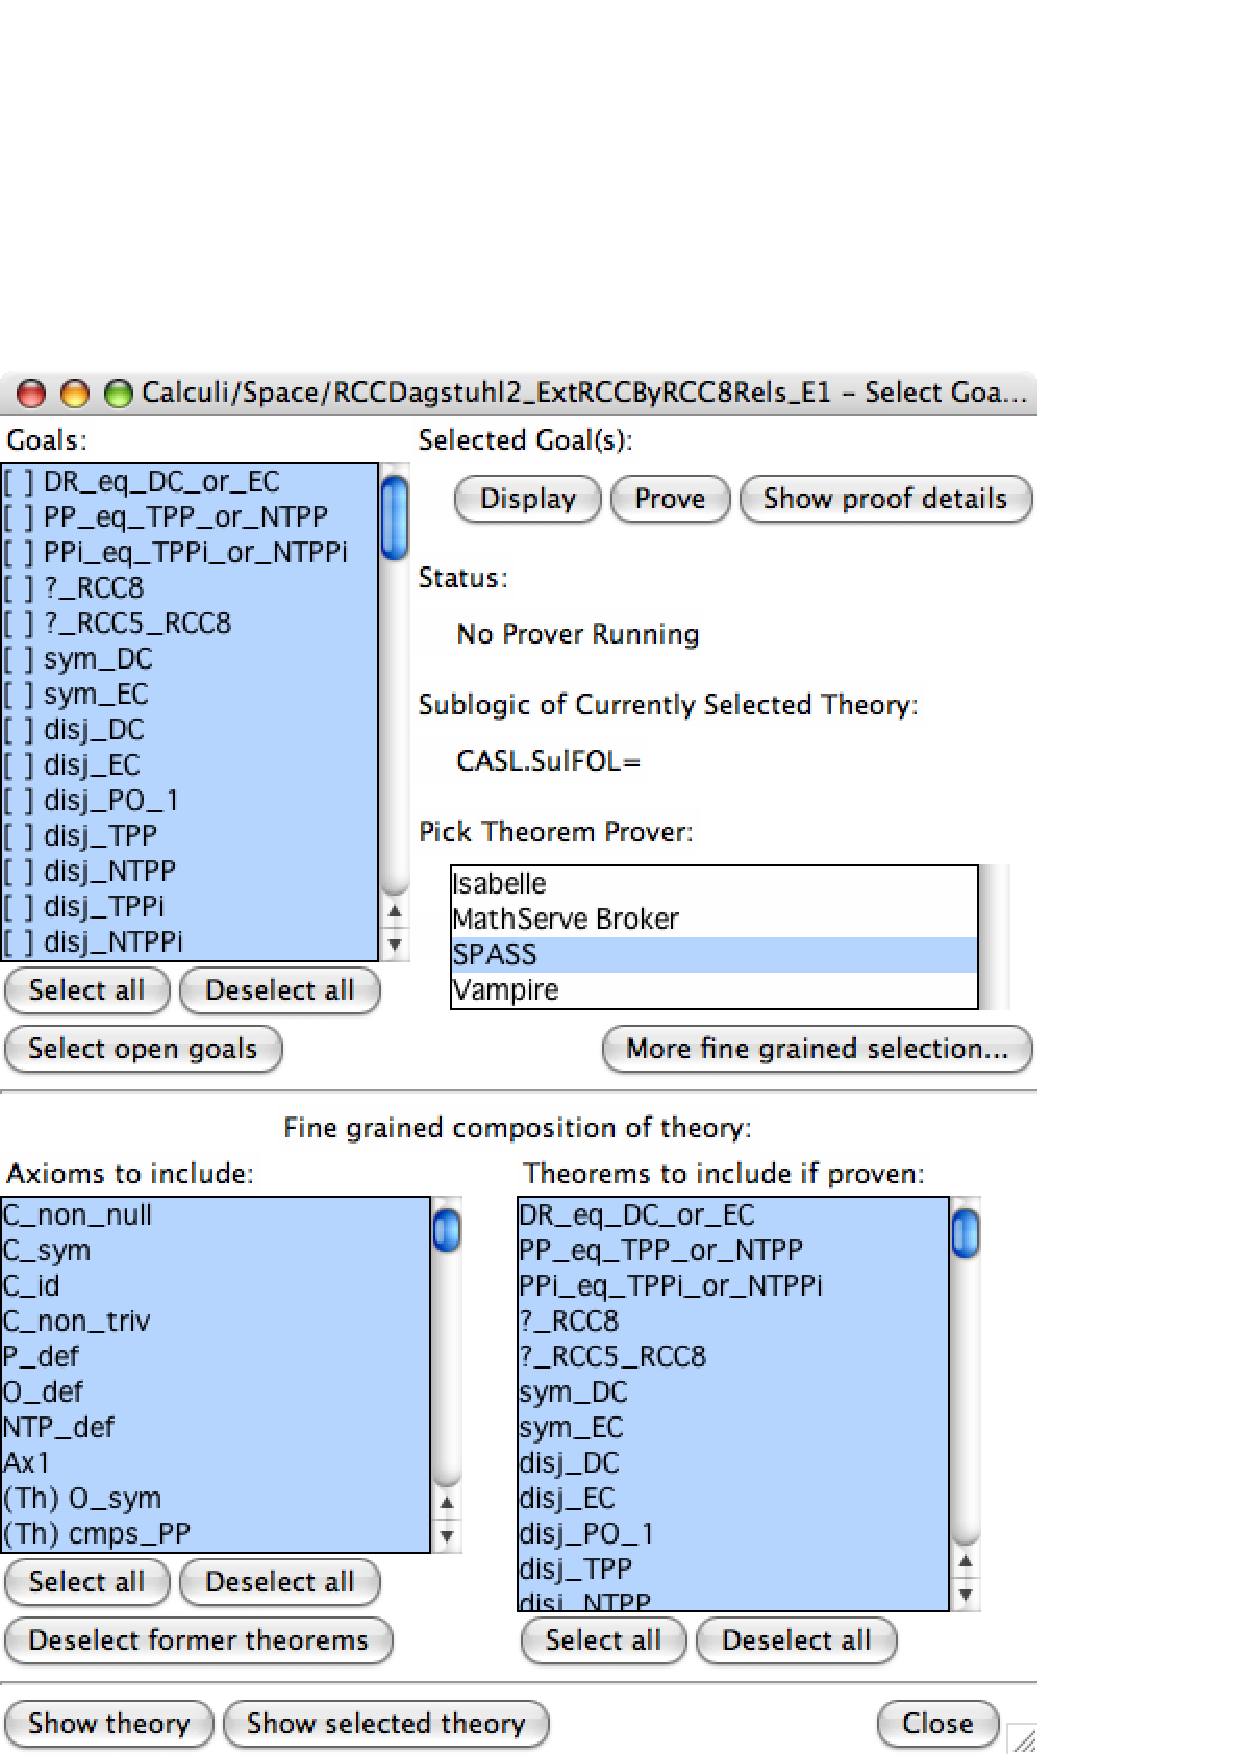
\includegraphics[width=\textwidth]{proofmanagement1}
\caption{Hets Goal and Prover Interface\label{fig:proof_window}}
\end{figure}

If you open this GUI when processing the goals of one node for the
first time, it will show all goals as open. Within this list you can
select those goals that should be inspected or proved. The button
`Display' shows the selected goals in the ASCII syntax of this
theory's logic in a separate window. With the `Prove' button the
actual prover is launched. This is described in more detail in the
paragraphs below. By pressing the `Show Proof Details' button a window
is opened where for each proved goal the used axioms, its proof
script, and its proof are shown --- the level of detail depends on the
used theorem prover. The `Status:' shows either `No prover running' or
`Waiting for prover' in black or blue. If you press the `Close' button
the window is closed and the status of the goals' list is integrated
into the development graph. If all goals have been proved, the
selected node turns from red into green.
\ednote{TODO Christian: describe disprove button}

\ednote{TODO Christian: describe consistency checker interface}


The list `Pick Theorem Prover:' lets you choose one of the connected
provers (among them \Isabelle, MathServe Broker, \SPASS,
Vampire, and zChaff, described below). By pressing `Prove' the
selected prover is launched and the theory along with the selected
goals is translated via the shortest possible path of comorphisms into
the provers logic.  The button `More fine grained selection...' lets
you pick a (composed) comorphism in a separate window from where the
prover is launched then.

Since the amount and kind of sentences sent to an ATP system is a
major factor for the performance of the ATP system, it is possible to
select the axioms and proven theorems that will comprise the theory
of the next proof attempt. Based on this selection the sublogic may
vary and also the available provers and comorphisms to provers. Former
theorems that are imported from other specifications are marked with
the prefix `(Th)'. Since former theorems do not add additional logical
content, they may be safely removed from the theory.

\subsection[Automated Theorem Proving Systems]
{Automated Theorem Proving Systems\\(Logic SoftFOL)}
\label{sec:ATP}

\begin{figure}
\centering
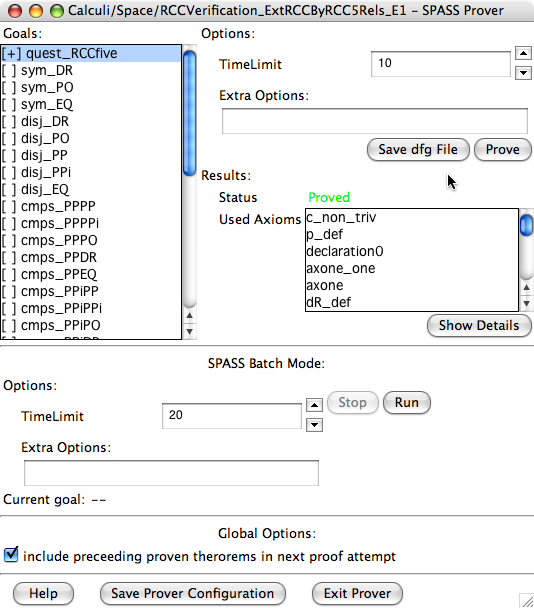
\includegraphics[width=\textwidth]{spassGUI1}
\caption{Interface of the \SPASS prover\label{fig:SPASS_GUI}}
\end{figure}

All ATPs integrated into \Hets share the same GUI, with only a slight
modification for the MathServe Broker: it does not have input
fields for extra options. Figure~\ref{fig:SPASS_GUI} shows the
instantiation for \SPASS, where in the lower part of the window the
batch mode can be controlled. The upper part shows on the left the
list of goals (with the same status indicators as in the Proof
Management GUI), and on the right a proof attempt of the selected goal
is controlled and the result of the last proof attempt is displayed.
The status line indicates `Open', `Running', `Proved', `Disproved',
`Open (Time is up!)', and `Proved (Theory inconsistent!)'. The list of
used axioms is actually only filled by \SPASS. The help button displays
information about the extra options accepted by the ATP system. The
button `Show Details' shows the whole output of the ATP system. `Save
Prover Configuration' allows you to save the configuration and status
of each proof for documentation. By pressing the button `Exit Prover'
the status of these proofs and goals is transferred back to the
Proof Management GUI.

The MathServe system \cite{ZimmerAutexier06} developed by J\"{u}rgen
Zimmer provides a unified interface to a range of different ATP
systems; the most important systems are listed in
Table~\ref{tab:MathServe}, along with their capabilities. These
capabilities are derived from the \emph{Specialist Problem Classes}
(SPCs) defined upon the basis of logical, language and syntactical
properties by Sutcliffe and Suttner \cite{SutcliffeEA:2001:EvalATP}.
Only two of the Web services provided by the MathServe system are used
by \Hets currently: Vampire and the brokering system.  The ATP systems
are offered as Web Services using standardized protocols and formats
such as SOAP, HTTP and XML.  Currently, the ATP system Vampire may be
accessed from \Hets via MathServe; the other systems are only reached
after brokering.

\begin{table}[t]
  \centering
  \begin{threeparttable}
    \begin{tabular}{|l|c|p{7cm}|}\firsthline
      ATP System & Version & Suitable Problem Classes\tnote{a}\\
      \hhline{|=|=|=|}
      DCTP & 10.21p & effectively propositional \\\hline
      EP & 0.91 & effectively propositional; real first-order, no
      equality; real first-order, equality\\\hline
      Otter & 3.3 & real first-order, no equality\\\hline
      \SPASS & 2.2 & effectively propositional; real first-order, no
      equality; real first-order, equality\\\hline
      Vampire & 8.0 & effectively propositional; pure equality, equality
      clauses contain non-unit equality clauses; real first-order, no
      equality, non-Horn\\\hline
      Waldmeister & 704 & pure equality, equality clauses are unit
      equality clauses\\\lasthline
    \end{tabular}
    %\renewcommand{\thempfootnote}{\arabic{mpfootnote}}
    %\footnotetext%[\value{footnote}\stepcounter{footnote}]
    \begin{tablenotes}\footnotesize
    \item[a]
      {The list of problem classes for each ATP system is not
        exhaustive, but only the most appropriate problem classes are
        named according to benchmark tests made with MathServe by
        J\"urgen Zimmer.}
    \end{tablenotes}
  \end{threeparttable}
  \caption{ATP systems provided as Web services by MathServe}
\vspace*{-4mm}
  \label{tab:MathServe}
\end{table}

\subsubsection*{\SPASS}

The ATP system \SPASS \cite{WeidenbachEtAl02} is a resolution-based
prover for first-order logic with equality. Furthermore, it provides a soft
typing mechanism with subsorting that treats sorts as unary
predicates. The ATP \SPASS should be installed locally and available
through your \verb,$PATH, environment variable.

\subsubsection*{Vampire}
% http://www.cs.miami.edu/~tptp/CASC/J3/SystemDescriptions.html#Vampire---8.0
The ATP system Vampire is the winner of the last 5 CADE ATP System
Competitions (CASC) (2002--2006) in the devisions \verb,FOF, and
\verb,CNF,. It is a resolution based ATP system supporting the calculi
of ordered binary resolution and superposition for handling equality.
See
\url{http://www.cs.miami.edu/~tptp/CASC/J3/SystemDescriptions.html#Vampire---8.0}
for detailed information. The connection to Vampire is achieved by
using an Web service of the MathServe system.

\subsubsection*{MathServe Broker}

% The classes ``effectively propositional'' and ``real first-order''
% apply to first-order problems that are distinguished by the finiteness
% of the Herbrand universe; an effectively propositional problem has
% only constants (generated by finitely many terms) whereas a real
% first-order problem contains true functions with an infinite Herbrand
% universe.
The brokering service chooses the most appropriate ATP system
upon a classification based on the SPCs, and on a training with the
library Thousands of Problems for Theorem Provers (TPTP)
\cite{ZimmerAutexier06}. The TPTP format
has been introduced by Sutcliffe and Suttner for the annual
competition CASC \cite{Sutcliffe:2006:CASC} and provides a unified
syntax for untyped FOL with equality, but without any symbol
declaration.

\subsection{Isabelle}

\Isabelle \cite{NipPauWen02} is an interactive theorem prover, which is
more powerful than ATP systems, but also requires more user interaction.

\Isabelle
has a very small core guaranteeing correctness, and its provers,
like the simplifier or the tableaux prover, are built on top of this
core. Furthermore, there is over fifteen years of experience with it,
and several mathematical textbooks have been partially
                \index{formal!verification}%
verified with
\Isabelle.

\Isabelle is a tactic based theorem prover implemented in standard ML.
The main \Isabelle logic (called Pure) is some weak intuitionistic type
theory with polymorphism. The logic Pure is used to represent a
variety of logics within \Isabelle; one of them being \HOL (higher-order
logic).  For example, logical implication in Pure (written
\texttt{==>}, also called meta-implication), is different from logical
implication in \HOL (written \texttt{-->}, also called object
implication).

It is essential to be aware of the fact that the \Isabelle/\HOL logic
is different from the logics that are encoded into it via comorphisms.
Therefore, the formulas appearing in subgoals of proofs with \Isabelle
will not conform to the syntax of the original input logic.  They may
even use features of \Isabelle/\HOL such as higher-order functions
that are not present in an input logic like \CASL.

\Isabelle is started with ProofGeneral
\cite{DBLP:conf/tacas/Aspinall00,url:ProofGeneral} in a separate Emacs
\cite{url:Emacs,url:XEmacs}.
The \Isabelle theory file conforms to the Isabelle/Isar syntax
\cite{NipPauWen02}. It starts with the theory (encoded along the selected
 comorphism), followed by a list of theorems. Initially, all the
 theorems have trivial proofs, using the `oops` command. However, if
 you have saved earlier proof attempts, \Hets will patch these into
 the generated \Isabelle theory file, ensuring that your previous work
 is not lost. (But note that this patching can only be successful
 if you do not rename specifications, or change their structure.)  You
 now can replace the 'oops' commands with real \Isabelle proofs, and
 use Proof General to step through the proofs. You finish your session
 by saving your file (using the Emacs file menu, or the Ctrl-x Ctrl-s
 key sequence), and by exiting Emacs (Ctrl-x Ctrl-c).


\subsection{VSE}
 The specification environment Verification Support Environment
(VSE) \cite{VSE00}, developed at
DFKI Saarbr\"ucken, provides an industrial-strength  methodology
for specification and verification of imperative programs.
VSE provides an interactive prover, which supports a Gentzen style
natural deduction calculus for dynamic logic.
This logic is an extension of first-order logic with two additional
kinds of formulas
that allow for reasoning about programs. One of them is the
box formula $[\alpha]\varphi$, where $\alpha$ is a program written in an imperative
language, and $\varphi$ is a dynamic logic formula.
The meaning of $[\alpha]\varphi$ can be roughly put as
``After every terminating execution of $\alpha$, $\varphi$ holds.''.
The other new kind
of formulas is the diamond formula $\langle\alpha\rangle\varphi$, which is the dual counter part
of a box formula. The meaning of $\langle\alpha\rangle\varphi$
can be described as ``After some terminating execution of $\alpha$,
$\varphi$ holds''.

\ednote{TODO Christian: describe interaction with \Hets}

\subsection{zChaff}

zChaff is a solver for satisfiabily problems of boolean formulas
(\normalTEXTSC{S}{AT})
in CNF. It is connected as a prover for propositional logic to \Hets. The prover
\SPASS is used to transform arbitrary boolean formulas to CNF. zChaff
implements the \normalTEXTSC{C}{HAFF}\xspace algorithm. We are
using the property, that a conjecture under the assumption of a set of axioms is
true, if the variables of axioms together with the negation of the conjecture
have no satisfying assignment, to prove theorems with zChaff. That is why you see
the result \normalTEXTSC{U}{NSAT}\xspace in the proof details, if a theorem has been proved
to be true. zChaff uses the same ATP GUI as the provers for SoftFOL (ref. to section
\ref{sec:ATP}). zChaff does not accept any options apart from the time-limit. The
current integration of zChaff into \Hets has been tested with zChaff 2004.11.15.

\subsection{Reduce}
\ednote{TODO : Dominik D.}
\subsection{Pellet}
Pellet is a popular open-source \DL-reasoner for \SROIQ, which is the logic
underlying OWL 2.0, written in Java. A Java Runtime Environment (in version > 1.5)
is needed to run Pellet. For the integration into \Hets the environment variable
\verb+PELLET_PATH+ has to be set to the root-directory of the Pellet installation.

Pellet uses the same ATP GUI as the provers for SoftFOL (ref. to section
\ref{sec:ATP}).
\subsection{Fact++}
Fact++ is a \DL-reasoner for \SROIQ, which is the logic underlying OWL 2.0, written in
C++. Fact++ is integrated into \Hets via the OWL-API, which is written in Java.
A Java Runtime Environment (in version >= 1.5) has to be installed. To use Fact++,
the environment variable \verb+HETS_OWL_TOOLS+ has to be set to the directory
containing the files
\begin{verbatim}
OWLFact.jar
OWLFactProver.jar
lib/FaCTpp-OWLAPI-v1.3.0.1.jar
lib/owlapi-bin.jar
\end{verbatim}
as well as
\begin{verbatim}
lib/native/i686/libFaCTPlusPlusJNI.so
\end{verbatim}
on a 32bits-Linux-system or
\begin{verbatim}
lib/native/x86_64/libFaCTPlusPlusJNI.so
\end{verbatim}
in a 64bits-Linux-system. Fact++ does not support options.

Fact++ uses the same ATP GUI as the provers for SoftFOL (ref. to section
\ref{sec:ATP}).
\subsection{QuickCheck}
\ednote{TODO Till}
\subsection{minisat}
\ednote{TODO Till}
\subsection{Truth tables}
\ednote{TODO Till}
\subsection{E-KRHyper}
E-KRHyper\footnote{\url{http://www.uni-koblenz.de/~bpelzer/ekrhyper/}}
is an extension of
KRHyper\footnote{\url{http://www.uni-koblenz.de/~wernhard/krhyper/}} by
handling of equality. E-KRHyper is an automatic first order theorem
prover and model finder based on the Hyper Tableaux Calculus\cite{Baumgartner:1996}.
E-KRHyper is optimized for being integrated into other systems. In the current
implementation we use a default tactics script, that can be influenced by the user.
The options of E-KRHyper are written in a Prolog-like syntax as in
\begin{verbatim}
#(set_parameter(timeout_termination_method,0)).
\end{verbatim}
the ``.'' at the end of each option is mandatory. To get an overview of
E-KRHyper's options, run the command
\begin{verbatim}
ekrh
\end{verbatim}
in a terminal. Then enter the command
\begin{verbatim}
#(help).
\end{verbatim}
at the prompt of E-KRHyper, to display its help information, which is basically
a long list of all available parameters. You can exit E-KRHyper by the command
\begin{verbatim}
#(exit).
\end{verbatim}

E-KRHyper uses the same ATP GUI as the other provers for SoftFOL (ref. to section
\ref{sec:ATP}).
\subsection{Darwin}
Darwin is an automatic first order prover and model finder implementing the Model
Evolution
Calculus\cite{Baumgartner:2003}. The integration of Darwin as a consistency checker
supports the display of models (if they can be constructed) in \CASL-syntax.
Eprover is needed to be in the system-path, if Darwin is used with \Hets, since
Darwin uses Eprover for clausification of first-order formulae.

Darwin supports a wide range of options, to get an overview of them run the command
\begin{verbatim}
darwin --help
\end{verbatim}
in a terminal.

Darwin uses the same ATP GUI as the other provers for SoftFOL (ref. to section
\ref{sec:ATP}).
\subsection{CspCASLProver}
\ednote{TODO Markus}


\section{Limits of Hets}

\Hets is still intensively under development. In particular, the
following points are still missing:

\begin{itemize}
\item There is no proof support for architectural specifications.
\item Distributed libraries are always downloaded from the local disk,
not from the Internet.
\item Version numbers of libraries are not considered properly.
\item The proof engine for development graphs provides only experimental
support for hiding links and for conservativity.
\end{itemize}


\section{Architecture of Hets}

The architecture of \Hets is shown in Fig.~\ref{fig:hets}.
How is a single logic implemented in the Heterogeneous Tool Set?
This is depicted in the left column of Fig.~\ref{fig:hets}.

\Hets provides an abstract interface for
                \index{institution!independence}%
                \index{independence, institution}%
institutions, so
that new logics can be integrated smoothly.
In order to do so, a parser,
a static checker and a prover for basic specifications in the logic have
to be provided.



\begin{figure}
%\figrule
\begin{center}
{\small
\begin{verbatim}
class Logic lid sign morphism sentence basic_spec symbol_map
    | lid -> sign morphism sentence basic_spec symbol_map where
  identity :: lid -> sign -> morphism
  compose :: lid -> morphism -> morphism -> morphism
  dom, codom :: lid -> morphism -> sign
  parse_basic_spec :: lid -> String -> basic_spec
  parse_symbol_map :: lid -> String -> symbol_map
  parse_sentence   :: lid -> String -> sentence
  empty_signature :: lid -> sign
  basic_analysis :: lid -> sign -> basic_spec -> (sign, [sentence])
  stat_symbol_map :: lid -> sign -> symbol_map -> morphism
  map_sentence :: lid -> morphism -> sentence -> sentence
  provers ::
    lid -> [(sign, [sentence]) -> [sentence] -> Proof_status]
  cons_checkers :: lid -> [(sign, [sentence]) -> Proof_status]

class Comorphism cid
          lid1 sign1 morphism1 sentence1 basic_spec1 symbol_map1
          lid2 sign2 morphism2 sentence2 basic_spec2 symbol_map2
      | cid -> lid1 lid2 where
  sourceLogic :: cid -> lid1       targetLogic :: cid -> lid2
  map_theory :: cid -> (sign1, [sentence1]) -> (sign2, [sentence2])
  map_morphism :: cid -> morphism1 -> morphism2
\end{verbatim}
}
\end{center}
\caption{The basic ingredients of logics and logic comorphisms}
\label{fig:logic:all}
%\figrule
\end{figure}

Each logic is realized in the programming language Haskell
\cite{PeytonJones03} by a set of types and functions, see
Fig.~\ref{fig:logic:all}, where we present a simplified, stripped down
version, where e.g.\ error handling is ignored. For technical reasons
a logic is \emph{tagged} with a unique identifier type (\texttt{lid}),
which is a singleton type the only purpose of which is to determine
all other type components of the given logic.  In Haskell jargon, the
interface is called a multiparameter type class with functional
dependencies \cite{TypeClasses}.  The Haskell interface for logic
translations is realised similarly.


The logic-independent modules in \Hets can be found in the right half
of Fig.~\ref{fig:hets}.  These modules comprise roughly one third of
\Hets' 100.000 lines of Haskell code.

The heterogeneous parser transforms a string
conforming to the syntax in Fig.~\ref{fig:lang}
to an abstract syntax tree, using the \texttt{Parsec} combinator parser
\cite{Parsec}.  Logic and translation names are looked up in the logic
graph --- this is necessary to be able to choose the correct parser
for basic specifications.  Indeed, the parser has a state that carries
the current logic, and which is updated if an explicit specification
of the logic is given, or if a logic translation is encountered (in
the latter case, the state is set to the target logic of the
translation).  With this, it is possible to parse basic specifications
by just using the logic-specific parser of the current logic as
obtained from the state.


The static analysis is based on the static analysis of basic
specifications, and transforms an abstract syntax tree to a
development graph (cf.\ Sect.~\ref{sec:DevGraph} above).  Starting with a
node corresponding to the empty theory, it successively extends (using
the static analysis of basic specifications) and/or translates (along
the intra- and inter-logic translations) the theory, while
simultaneously adding nodes and links to the development graph.

Heterogeneous proof management is done using heterogeneous
development graphs, as described in Sect.~\ref{sec:DevGraph}.
For local proof goals, logic-specific provers are invoked,
see Sect.~\ref{sec:Proofs}.

\Hets can store development graphs, including their proofs.
Therefore, \Hets uses the so-called
                \index{ATerms}%
ATerm format \cite{BJKO00}, which is used as interchange format
for interfacing with other tools.

More details can be found in \cite{Habil,MossakowskiEtAl07b}
and in the overview of modules provided in the developers section
of the \Hets home page at \url{http://www.dfki.de/sks/hets}.

\begin{figure}
\begin{center}
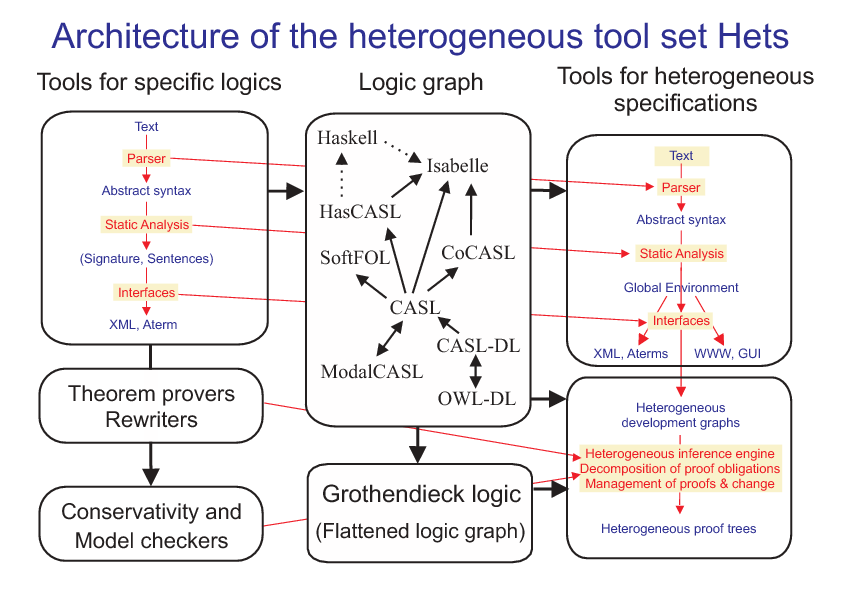
\includegraphics[scale=0.4]{hets2007}
\end{center}
%\vspace{1em}
%\setlength{\unitlength}{1740sp}%
%
\begingroup\makeatletter\ifx\SetFigFont\undefined%
\gdef\SetFigFont#1#2#3#4#5{%
  \reset@font\fontsize{#1}{#2pt}%
  \fontfamily{#3}\fontseries{#4}\fontshape{#5}%
  \selectfont}%
\fi\endgroup%
\begin{picture}(12534,8879)(439,-8907)
\thinlines
{\color[rgb]{0,0,0}\put(2458,-5596){\vector( 0,-1){630}}
}%
{\color[rgb]{0,0,0}\put(2458,-4799){\vector( 0,-1){270}}
}%
{\color[rgb]{0,0,0}\put(2458,-4269){\line( 0,-1){260}}
}%
{\color[rgb]{0,0,0}\put(2458,-3645){\vector( 0,-1){270}}
}%
{\color[rgb]{0,0,0}\put(2458,-3115){\line( 0,-1){260}}
}%
{\color[rgb]{0,0,0}\put(2458,-2491){\vector( 0,-1){270}}
}%
{\color[rgb]{0,0,0}\put(2458,-1961){\line( 0,-1){260}}
}%
{\color[rgb]{0,0,0}\put(10773,-5551){\vector( 0,-1){900}}
}%
{\color[rgb]{0,0,0}\put(10773,-4799){\vector( 0,-1){270}}
}%
{\color[rgb]{0,0,0}\put(10773,-4269){\line( 0,-1){260}}
}%
{\color[rgb]{0,0,0}\put(10773,-3645){\vector( 0,-1){270}}
}%
{\color[rgb]{0,0,0}\put(10773,-3115){\line( 0,-1){260}}
}%
{\color[rgb]{0,0,0}\put(10773,-2491){\vector( 0,-1){270}}
}%
{\color[rgb]{0,0,0}\put(10773,-1961){\line( 0,-1){260}}
}%
{\color[rgb]{0,0,0}\put(6436,-3391){\line(-2, 3){595.385}}
}%
{\color[rgb]{0,0,0}\put(6571,-3391){\line( 0, 1){1530}}
}%
{\color[rgb]{0,0,0}\put(6706,-3391){\line( 2, 3){595.385}}
}%
{\color[rgb]{0,0,0}\put(7039,-3523){\line( 3, 2){488.077}}
}%
{\color[rgb]{0,0,0}\put(6226,-3548){\line(-3, 2){488.077}}
}%
{\color[rgb]{0,0,0}\put(5791,-4046){\line( 3, 2){405}}
}%
{\color[rgb]{0,0,0}\put(7253,-4056){\line(-3, 2){405}}
}%
{\color[rgb]{0,0,0}\put(6795,-4557){\line( 5, 2){411.207}}
}%
{\color[rgb]{0,0,0}\put(6283,-4558){\line(-5, 2){411.207}}
}%
{\color[rgb]{0,0,0}\put(5691,-5146){\line( 3, 2){405}}
}%
{\color[rgb]{0,0,0}\put(7403,-5146){\line(-3, 2){405}}
}%
{\color[rgb]{0,0,0}\put(6571,-5056){\line( 0, 1){180}}
}%
{\color[rgb]{0,0,0}\put(10773,-2755){\oval(3785,5632)}
%\put(9106,-164){\oval(210,210)[tl]}
%\put(12541,-5446){\oval(210,210)[br]}
%\put(12541,-164){\oval(210,210)[tr]}
%\put(9106,-5551){\line( 1, 0){3435}}
%\put(9106,-59){\line( 1, 0){3435}}
%\put(9001,-5446){\line( 0, 1){5282}}
%\put(12646,-5446){\line( 0, 1){5282}}
}%
{\color[rgb]{0,0,0}\put(2458,-2755){\oval(3785,5632)}
%{\color[rgb]{0,0,0}\put(781,-5491){\oval(210,210)[bl]}
%\put(781,-145){\oval(210,210)[tl]}
%\put(4306,-5491){\oval(210,210)[br]}
%\put(4306,-145){\oval(210,210)[tr]}
%\put(781,-5596){\line( 1, 0){3525}}
%\put(781,-40){\line( 1, 0){3525}}
%\put(676,-5491){\line( 0, 1){5346}}
%\put(4411,-5491){\line( 0, 1){5346}}
}%
{\color[rgb]{0,0,0}\put(6623,-2755){\oval(3785,5632)}
%{\color[rgb]{0,0,0}\put(4966,-5491){\oval(210,210)[bl]}
%\put(4966,-166){\oval(210,210)[tl]}
%\put(8430,-5491){\oval(210,210)[br]}
%\put(8430,-166){\oval(210,210)[tr]}
%\put(4966,-5596){\line( 1, 0){3464}}
%\put(4966,-61){\line( 1, 0){3464}}
%\put(4861,-5491){\line( 0, 1){5325}}
%\put(8535,-5491){\line( 0, 1){5325}}
}%
{\color[rgb]{0,0,0}\put(4361,-2851){\line( 1, 0){350}}
}%
{\color[rgb]{0,0,0}\put(8521,-2851){\vector( 1, 0){350}}
}%
{\color[rgb]{0,0,0}\put(751,-7276){\oval(330,330)[bl]}
\put(751,-6526){\oval(330,330)[tl]}
\put(2941,-7276){\oval(330,330)[br]}
\put(2941,-6526){\oval(330,330)[tr]}
\put(751,-7441){\line( 1, 0){2190}}
\put(751,-6361){\line( 1, 0){2190}}
\put(586,-7276){\line( 0, 1){750}}
\put(3106,-7276){\line( 0, 1){750}}
}%
{\color[rgb]{0,0,0}\put(586,-8760){\oval(270,270)[bl]}
\put(586,-6361){\oval(270,270)[tl]}
\put(5851,-8760){\oval(270,270)[br]}
\put(5851,-6361){\oval(270,270)[tr]}
\put(586,-8895){\line( 1, 0){5265}}
\put(586,-6226){\line( 1, 0){5265}}
\put(451,-8760){\line( 0, 1){2399}}
\put(5986,-8760){\line( 0, 1){2399}}
}%
{\color[rgb]{0,0,0}\put(1726,-8551){\oval(300,300)[bl]}
\put(1726,-7906){\oval(300,300)[tl]}
\put(4411,-8551){\oval(300,300)[br]}
\put(4411,-7906){\oval(300,300)[tr]}
\put(1726,-8701){\line( 1, 0){2685}}
\put(1726,-7756){\line( 1, 0){2685}}
\put(1576,-8551){\line( 0, 1){645}}
\put(4561,-8551){\line( 0, 1){645}}
}%
{\color[rgb]{0,0,0}\put(8537,-8101){\oval(300,300)[bl]}
\put(8537,-6646){\oval(300,300)[tl]}
\put(12811,-8101){\oval(300,300)[br]}
\put(12811,-6646){\oval(300,300)[tr]}
\put(8537,-8251){\line( 1, 0){4274}}
\put(8537,-6496){\line( 1, 0){4274}}
\put(8387,-8101){\line( 0, 1){1455}}
\put(12961,-8101){\line( 0, 1){1455}}
}%
{\color[rgb]{0,0,0}\put(3481,-7290){\oval(300,300)[bl]}
\put(3481,-6531){\oval(300,300)[tl]}
\put(5656,-7290){\oval(300,300)[br]}
\put(5656,-6531){\oval(300,300)[tr]}
\put(3481,-7440){\line( 1, 0){2175}}
\put(3481,-6381){\line( 1, 0){2175}}
\put(3331,-7290){\line( 0, 1){759}}
\put(5806,-7290){\line( 0, 1){759}}
}%
{\color[rgb]{0,0,0}\put(5986,-7441){\vector( 1, 0){2385}}
}%
\put(2135,-1861){\makebox(0,0)[lb]{\smash{\SetFigFont{7}{8.4}{\sfdefault}{\mddefault}{\updefault}{\color[rgb]{0,0,0}Text}%
}}}
\put(2106,-2438){\makebox(0,0)[lb]{\smash{\SetFigFont{7}{8.4}{\sfdefault}{\mddefault}{\updefault}{\color[rgb]{0,0,0}\emph{Parser}}%
}}}
\put(1441,-3015){\makebox(0,0)[lb]{\smash{\SetFigFont{7}{8.4}{\sfdefault}{\mddefault}{\updefault}{\color[rgb]{0,0,0}Abstract syntax}%
}}}
\put(1616,-3592){\makebox(0,0)[lb]{\smash{\SetFigFont{7}{8.4}{\sfdefault}{\mddefault}{\updefault}{\color[rgb]{0,0,0}\emph{Static analysis}}%
}}}
\put(1131,-4169){\makebox(0,0)[lb]{\smash{\SetFigFont{7}{8.4}{\sfdefault}{\mddefault}{\updefault}{\color[rgb]{0,0,0}(Signature, Sentences)}%
}}}
\put(1896,-4746){\makebox(0,0)[lb]{\smash{\SetFigFont{7}{8.4}{\sfdefault}{\mddefault}{\updefault}{\color[rgb]{0,0,0}\emph{Interfaces}}%
}}}
\put(1641,-5323){\makebox(0,0)[lb]{\smash{\SetFigFont{7}{8.4}{\sfdefault}{\mddefault}{\updefault}{\color[rgb]{0,0,0}XML, ATerms}%
}}}
\put(6301,-3706){\makebox(0,0)[lb]{\smash{\SetFigFont{7}{8.4}{\sfdefault}{\mddefault}{\updefault}{\color[rgb]{0,0,0}CASL}%
}}}
\put(5356,-2356){\makebox(0,0)[lb]{\smash{\SetFigFont{7}{8.4}{\sfdefault}{\mddefault}{\updefault}{\color[rgb]{0,0,0}CoCASL}%
}}}
\put(6976,-2356){\makebox(0,0)[lb]{\smash{\SetFigFont{7}{8.4}{\sfdefault}{\mddefault}{\updefault}{\color[rgb]{0,0,0}CASL-LTL}%
}}}
\put(6121,-1726){\makebox(0,0)[lb]{\smash{\SetFigFont{7}{8.4}{\sfdefault}{\mddefault}{\updefault}{\color[rgb]{0,0,0}CSP-CASL}%
}}}
\put(7201,-3121){\makebox(0,0)[lb]{\smash{\SetFigFont{7}{8.4}{\sfdefault}{\mddefault}{\updefault}{\color[rgb]{0,0,0}SB-CASL}%
}}}
\put(5041,-3166){\makebox(0,0)[lb]{\smash{\SetFigFont{7}{8.4}{\sfdefault}{\mddefault}{\updefault}{\color[rgb]{0,0,0}HasCASL}%
}}}
\put(5086,-4336){\makebox(0,0)[lb]{\smash{\SetFigFont{7}{8.4}{\sfdefault}{\mddefault}{\updefault}{\color[rgb]{0,0,0}SubFOL$^=$}%
}}}
\put(7246,-4336){\makebox(0,0)[lb]{\smash{\SetFigFont{7}{8.4}{\sfdefault}{\mddefault}{\updefault}{\color[rgb]{0,0,0}PFOL$^=$}%
}}}
\put(6346,-4786){\makebox(0,0)[lb]{\smash{\SetFigFont{7}{8.4}{\sfdefault}{\mddefault}{\updefault}{\color[rgb]{0,0,0}FOL$^=$}%
}}}
\put(6346,-5371){\makebox(0,0)[lb]{\smash{\SetFigFont{7}{8.4}{\sfdefault}{\mddefault}{\updefault}{\color[rgb]{0,0,0}Horn$^=$}%
}}}
\put(5400,-5371){\makebox(0,0)[lb]{\smash{\SetFigFont{7}{8.4}{\sfdefault}{\mddefault}{\updefault}{\color[rgb]{0,0,0}$\bullet$}%
}}}
\put(7600,-5371){\makebox(0,0)[lb]{\smash{\SetFigFont{7}{8.4}{\sfdefault}{\mddefault}{\updefault}{\color[rgb]{0,0,0}$\bullet$}%
}}}
\put(1006,-421){\makebox(0,0)[lb]{\smash{\SetFigFont{7}{8.4}{\rmdefault}{\bfdefault}{\updefault}{\color[rgb]{0,0,0}Basic specifications}%
}}}
\put(826,-826){\makebox(0,0)[lb]{\smash{\SetFigFont{7}{8.4}{\rmdefault}{\bfdefault}{\updefault}{\color[rgb]{0,0,0}(logic-specific tools for}%
}}}
\put(826,-1231){\makebox(0,0)[lb]{\smash{\SetFigFont{7}{8.4}{\rmdefault}{\bfdefault}{\updefault}{\color[rgb]{0,0,0}CASL and extensions)}%
}}}
\put(5411,-421){\makebox(0,0)[lb]{\smash{\SetFigFont{7}{8.4}{\rmdefault}{\bfdefault}{\updefault}{\color[rgb]{0,0,0}Graph of CASL}%
}}}
\put(9591,-421){\makebox(0,0)[lb]{\smash{\SetFigFont{7}{8.4}{\rmdefault}{\bfdefault}{\updefault}{\color[rgb]{0,0,0}Structured and}%
}}}
\put(9771,-826){\makebox(0,0)[lb]{\smash{\SetFigFont{7}{8.4}{\rmdefault}{\bfdefault}{\updefault}{\color[rgb]{0,0,0}architectural}%
}}}
\put(9796,-1231){\makebox(0,0)[lb]{\smash{\SetFigFont{7}{8.4}{\rmdefault}{\bfdefault}{\updefault}{\color[rgb]{0,0,0}specifications}%
}}}
\put(10501,-1861){\makebox(0,0)[lb]{\smash{\SetFigFont{7}{8.4}{\sfdefault}{\mddefault}{\updefault}{\color[rgb]{0,0,0}Text}%
}}}
\put(10441,-2428){\makebox(0,0)[lb]{\smash{\SetFigFont{7}{8.4}{\sfdefault}{\mddefault}{\updefault}{\color[rgb]{0,0,0}\emph{Parser}}%
}}}
\put(9886,-3015){\makebox(0,0)[lb]{\smash{\SetFigFont{7}{8.4}{\sfdefault}{\mddefault}{\updefault}{\color[rgb]{0,0,0}Abstract syntax}%
}}}
\put(9936,-3592){\makebox(0,0)[lb]{\smash{\SetFigFont{7}{8.4}{\sfdefault}{\mddefault}{\updefault}{\color[rgb]{0,0,0}\emph{Static analysis}}%
}}}
\put(9641,-4169){\makebox(0,0)[lb]{\smash{\SetFigFont{7}{8.4}{\sfdefault}{\mddefault}{\updefault}{\color[rgb]{0,0,0}Development graph}%
}}}
\put(10216,-4746){\makebox(0,0)[lb]{\smash{\SetFigFont{7}{8.4}{\sfdefault}{\mddefault}{\updefault}{\color[rgb]{0,0,0}\emph{Interfaces}}%
}}}
\put(9946,-5323){\makebox(0,0)[lb]{\smash{\SetFigFont{7}{8.4}{\sfdefault}{\mddefault}{\updefault}{\color[rgb]{0,0,0}XML, ATerms}%
}}}
\put(2476,-8476){\makebox(0,0)[lb]{\smash{\SetFigFont{7}{8.4}{\sfdefault}{\mddefault}{\updefault}{\color[rgb]{0,0,0}(e.g. CCC)}%
}}}
\put(1936,-8161){\makebox(0,0)[lb]{\smash{\SetFigFont{7}{8.4}{\sfdefault}{\mddefault}{\updefault}{\color[rgb]{0,0,0}Consistency checker}%
}}}
\put(846,-7171){\makebox(0,0)[lb]{\smash{\SetFigFont{7}{8.4}{\sfdefault}{\mddefault}{\updefault}{\color[rgb]{0,0,0}(e.g. HOL-CASL)}%
}}}
\put(936,-6766){\makebox(0,0)[lb]{\smash{\SetFigFont{7}{8.4}{\sfdefault}{\mddefault}{\updefault}{\color[rgb]{0,0,0}Theorem prover}%
}}}
\put(8806,-7846){\makebox(0,0)[lb]{\smash{\SetFigFont{7}{8.4}{\sfdefault}{\mddefault}{\updefault}{\color[rgb]{0,0,0}Management of proofs \& change}%
}}}
\put(9091,-7351){\makebox(0,0)[lb]{\smash{\SetFigFont{7}{8.4}{\sfdefault}{\mddefault}{\updefault}{\color[rgb]{0,0,0}Heterogeneous proof engine}%
}}}
\put(10206,-6946){\makebox(0,0)[lb]{\smash{\SetFigFont{7}{8.4}{\rmdefault}{\bfdefault}{\updefault}{\color[rgb]{0,0,0}MAYA}%
}}}
\put(3501,-7216){\makebox(0,0)[lb]{\smash{\SetFigFont{7}{8.4}{\sfdefault}{\mddefault}{\updefault}{\color[rgb]{0,0,0}(e.g. ELAN-CASL)}%
}}}
\put(4051,-6766){\makebox(0,0)[lb]{\smash{\SetFigFont{7}{8.4}{\sfdefault}{\mddefault}{\updefault}{\color[rgb]{0,0,0}Rewriter}%
}}}
\put(5106,-1231){\makebox(0,0)[lb]{\smash{\SetFigFont{7}{8.4}{\rmdefault}{\bfdefault}{\updefault}{\color[rgb]{0,0,0}proposed extensions}%
}}}
\put(5280,-826){\makebox(0,0)[lb]{\smash{\SetFigFont{7}{8.4}{\rmdefault}{\bfdefault}{\updefault}{\color[rgb]{0,0,0}sublanguages and}%
}}}
\end{picture}

\caption{Architecture of the heterogeneous tool set.
\label{fig:hets}}
\end{figure}

\bigskip

\Hets is mainly maintained by
Christian Maeder (Christian.Maeder@dfki.de) and Till Mossakowski
(Till.Mossakowski@dfki.de). The mailing list is
\begin{quote}
 \url{hets-users@informatik.uni-bremen.de}
\end{quote}
the homepage is
\begin{quote}
\url{http://www.informatik.uni-bremen.de/mailman/listinfo/hets-users}.
\end{quote}

You need to subscribe to the list before you can send a mail.
But note that subscription is very easy!

If your favourite logic is missing in \Hets, please tell us
(hets-users@informatik.uni-bremen.de). We will take account your
feedback when deciding which logics and proof tools to integrate next
into \Hets. Help with integration of more logics and proof tools into
\Hets is also welcome.

\paragraph{Acknowledgement}
The heterogeneous tool set \Hets would not have possible
without cooperation with many people.
%Christian Maeder and Klaus L\"uttich.
Besides the authors, the following people have been involved
in the implementation of \Hets:
Katja Abu-Dib,
Mihai Codescu,
Carsten Fischer,
Jorina Freya Gerken,
Rainer Grabbe,
Sonja Gr\"{o}ning,
Daniel Hausmann,
Wiebke Herding,
Hendrik Iben,
Cui ``Ken'' Jian,
Heng Jiang,
Anton Kirilov,
Tina Krausser,
Martin K\"{u}hl,
Mingyi Liu,
Dominik L\"{u}cke,
%Klaus L\"{u}ttich,
%Christian Maeder,
Maciek Makowski,
Immanuel Normann,
Razvan Pascanu,
Daniel Pratsch,
Felix Reckers,
Markus Roggenbach,
Pascal Schmidt,
Paolo Torrini,
Ren\'{e} Wagner,
Jian Chun Wang and
Thiemo Wiedemeyer.

\Hets has been built based on experiences with its
precursors,
                \index{Cats@\Cats}%
\Cats and
                \index{Maya@\MAYA}%
\MAYA.
The \CASL Tool Set (\Cats)
\cite{Mossakowski:2000:CST,Mossakowski:1998:SSA}
provides parsing and static analysis for \CASL.
It has been developed by the first author with help
of Mark van den Brand, Kolyang, Bartek Klin, Pascal Schmidt and
Frederic Voisin.

\MAYA \cite{Autexier:2002:IHD,AutexierEtal02} is a proof management
tool based on development graphs.  \MAYA only supports development
graphs without hiding and without logic translations.  \MAYA has been
developed by Serge Autexier and Dieter Hutter.

We also want to thank Agn\`es Arnould, Thibaud Brunet, Pascale LeGall,
Kathrin Hoffmann, Katiane Lopes,
%Klaus L\"uttich, Christian Maeder,
Stefan Merz, Maria Martins Moreira, Christophe
Ringeissen, Markus Roggenbach, Dmitri Schamschurko, Lutz Schr\"oder,
Konstantin Tchekine and Stefan W\"olfl
for giving feedback about \Cats, HOL-CASL and \Hets. Finally,
special thanks to Christoph L\"uth and George Russell
for help with connecting \Hets to their UniForM workbench.


\bibliographystyle{plain}
\bibliography{cofibib,cofi-ann,UM,hets,kl}
\end{document}



%%% Local Variables:
%%% mode: latex
%%% TeX-master: "UserGuide"
%%% End:
